\documentclass[11pt,letterpaper]{article}

\usepackage[margin=1in]{geometry}
\usepackage{amsmath,amssymb}
\usepackage[T1]{fontenc}
\usepackage[round,authoryear]{natbib}
\usepackage{graphicx}
\usepackage{booktabs}
\usepackage{tabularx}
\usepackage{float}
\usepackage{hyperref}
\usepackage{caption}
\usepackage{subcaption}
\usepackage{enumitem}
\usepackage{multirow}

\title{Climate Volatility, Agricultural Pathway, and Modern Demographic Outcomes\\
{\large A Cross-Country Investigation Across Pre-Industrial and Modern Windows}}

\author{Jorge Alonso Ortiz\thanks{Centro de Investigaci\'on Econ\'omica, ITAM. Email: \texttt{jorge.alonso@itam.mx}.}
  \and Jos\'e-Mar\'ia Da-Rocha\thanks{Universidade de Vigo, RGEA, Spain.}}
\date{Draft: May 2026}

\begin{document}
\maketitle

\begin{abstract}
\noindent
A country-level panel is assembled of four pre-industrial channels of long-run development---a four-element climate bundle (mean temperature, mean precipitation, inter-annual temperature volatility $\sigma_v^T$, and inter-annual precipitation volatility $\sigma_v^P$, all over 1421--1750 from the ModE-RA paleo-reanalysis), ancestry-adjusted predicted heterozygosity \citep{ashraf2013out}, ancestral crop-yield potential \citep{galor2016agricultural}, and pre-1500 pandemic intensity---and used to investigate how each shapes a six-outcome vector that spans the Malthusian-to-post-Malthusian transition: log population density in 1500 CE (Malthusian-era proxy), log population density in 2025 (cumulative-productivity proxy), log population growth 1950--2025, urbanisation-share change 1950--2025, log GDP per capita 2015, and demographic-transition timing. The headline empirical object is a Shapley-Owen R\textsuperscript{2} decomposition on 185 countries, with the climate bundle treated as a coalition player. Five Westfall-Young FWER-corrected cells survive at $p<0.05$ across the 24-cell mediation matrix. Ancestral crop yield is the dominant predictor of modern population growth ($\hat\phi^{\text{Shap}}=0.122$, $F=27.0$, $p_{\text{WY}}<0.001$) and a robust predictor of population density at 1500 ($F=15.5$, $p_{\text{WY}}=0.002$) and 2025 ($F=10.4$, $p_{\text{WY}}=0.022$), spanning the full demographic-density trajectory. Predicted heterozygosity dominates log GDP per capita ($F=11.3$, $p_{\text{WY}}=0.015$) and is a robust secondary predictor of population growth ($F=10.8$, $p_{\text{WY}}=0.019$). The climate bundle contributes the largest Shapley R\textsuperscript{2} on three of the six outcomes (population density 1500, urbanisation change, and demographic-transition timing) but no climate cell survives FWER correction once pathway dummies enter the regression: its mediation share on density 1500 is 0.75 and on population growth is 0.92, consistent with the climate channel operating through pathway selection rather than as a direct channel. Within the climate bundle, $\sigma_v^T$ specifically drives the 1500-density contribution (0.042 of the bundle's 0.065 Shapley R\textsuperscript{2}), while mean precipitation drives the modern population-growth and urbanisation contributions, consistent with a Matranga-style storage mechanism that mattered for pre-industrial Malthusian dynamics and a separate water-availability channel shaping modern outcomes. Pathway mediation is well-behaved once continent fixed effects partial out continental heterogeneity. The five FWER-surviving findings are robust to climate-window placebos, cumulative conflict-exposure and volcanic-radiative-forcing controls, and a climate-A partialling that breaks the GAEZ-implied ($\bar T$, $\bar P$) correlation between ancestral crop yield and the climate bundle. On the 79-country Eurasian sub-sample with ancient-DNA-derived ancestry decompositions \citep{lazaridis2014,haak2015}, the heterozygosity signal on per-capita income is largely absorbed by Anatolian Neolithic farmer and Yamnaya steppe-pastoralist ancestry shares. The investigation places four pre-existing causal-identification literatures on a single panel and reveals that channels matter at different temporal moments: climate at the Malthusian steady state via pathway mediation, ancestral crop yield across the whole density trajectory, and predicted heterozygosity at the per-capita income margin.

\medskip
\noindent\textbf{JEL Codes:} O11, O13, O44, N50, Q54.\\
\textbf{Keywords:} Climate bundle, deep determinants, unified growth theory, population density, heterozygosity, ancestral crop yield, pandemic intensity, Shapley decomposition.
\end{abstract}

\section{Introduction}
\label{sec:intro}

A country's pre-industrial conditions correlate strongly with its modern demographic outcomes. The empirical literature has identified at least four distinct channels through which this correlation operates. \citet{ashraf2013out} argue that the ancestral genetic diversity of a country's population, predicted by the out-of-Africa migration history of its constituent ancestral populations and ancestry-adjusted to year-2000 composition \citep{putterman2010}, drives an inverted-U relationship with development. \citet{galor2016agricultural} argue that the ancestral suitability of a country's land for pre-1500 cultivated crops, measured from Global Agro-Ecological Zones (GAEZ) projections under pre-Columbian climate, shapes long-run economic outcomes through its effect on time-preference selection. The Voigtl\"ander-Voth post-Black-Death literature \citep{voigtlander2013how} argues that pre-1500 pandemic exposure had persistent effects on factor ratios and subsequent demographic-economic trajectories. The companion paper \citep{alonso_long_shadow}---hereafter LS---argues that pre-industrial inter-annual climate volatility 1421--1750 selected agricultural pathways and through them shaped both pre-industrial Malthusian dynamics and the modern demographic record. We treat the climate channel as a four-element bundle---mean temperature $\bar T$, mean precipitation $\bar P$, inter-annual temperature volatility $\sigma_v^T$, and inter-annual precipitation volatility $\sigma_v^P$, all over 1421--1750---rather than reducing it to $\sigma_v^T$ alone, both to put the climate channel on equal footing with the other three substrates (each of which is itself an index summarising multiple primitives) and because the Matranga (2024) storage mechanism that motivates the climate channel concerns the full bundle.

Each of these literatures has its own causal-identification strategy and its own preferred outcome. Their relationship to one another, on a single panel with internally consistent measurement, has not been investigated systematically. Several questions follow naturally. Does the climate bundle's predictive contribution survive once ancestral genetic diversity and ancestral crop-yield potential are conditioned in the same regression? Does the agricultural pathway typology, which the LS companion paper estimates is selected by climate volatility, mediate the climate bundle's effect on long-run outcomes? Do the four channels matter at different points in the Malthusian-to-post-Malthusian transition---some for pre-industrial population density, others for post-industrial per-capita income?

This paper investigates these questions on a 196-country panel that joins the climate bundle with canonical implementations of the three other deep-determinants channels and six outcomes spanning the demographic transition: log population density in 1500 CE (Malthusian-era proxy), log population density in 2025 (cumulative-productivity proxy), log population growth 1950--2025, urbanisation-share change 1950--2025, log GDP per capita 2015, and demographic-transition timing. The first two outcomes are drawn from HYDE 3.5 \citep{goldewijk2017}; the latter four from UN WPP, WUP, Maddison, and Gapminder/OWID sources. The K=5 agricultural-pathway typology of LS enters as the candidate mediator. We frame the exercise as an \emph{investigation} rather than a horserace with a designated winner: each of the four channels has its own causal-identification literature and we borrow their assumptions rather than re-litigate them. The contribution is to put them side-by-side and ask which of them carries unique-variance weight on which outcomes, conditional on the others, and how the climate bundle specifically relates to each.

Five findings survive Westfall-Young family-wise error-rate correction across the 24 substrate-by-outcome cells of the mediation matrix:

\emph{First, ancestral crop-yield potential is the dominant predictor of modern population growth, and a robust predictor of population density at both 1500 and 2025---spanning the full demographic-density trajectory.} On log population growth 1950--2025 the Shapley R\textsuperscript{2} is 0.122 and the FWER-corrected joint $F$-statistic on the mediated coefficient is 27.0 ($p_{\text{WY}}<0.001$), the largest single cell in the matrix. On log population density 1500 the Shapley R\textsuperscript{2} is 0.049 ($F=15.5$, $p_{\text{WY}}=0.002$); on log population density 2025 it is 0.023 ($F=10.4$, $p_{\text{WY}}=0.022$). Together these findings extend the Galor-\"Ozak (2016) result---originally framed through the time-preference channel---to the cross-country demographic-density trajectory: pre-1500 caloric potential of cultivable crops predicts population density at the Malthusian steady state, at the post-industrial steady state, and the convergence path that connects them.

\emph{Second, ancestry-adjusted predicted heterozygosity is the dominant predictor of modern log GDP per capita} (Shapley R\textsuperscript{2} 0.038, $F=11.3$, $p_{\text{WY}}=0.015$) \emph{and a robust secondary predictor of log population growth} ($F=10.8$, $p_{\text{WY}}=0.019$). The result for log GDP per capita reproduces the Ashraf-Galor (2013) headline finding in a panel that conditions on competing pre-industrial channels; the result for population growth is, to our knowledge, new. Section~\ref{sec:genetic-controls} shows that on the 79-country Eurasian sub-sample with ancient-DNA-derived ancestry decompositions \citep{lazaridis2014,haak2015}, this heterozygosity signal on per-capita income is largely absorbed by the Anatolian Neolithic farmer and Yamnaya steppe-pastoralist ancestry shares: the coefficient on $H$ moves from $-10.68$ (se 10.61) to $-1.70$ (se 13.11). The pattern is consistent with the migratory-distance heterozygosity measure proxying, within Eurasia, for which pre-industrial technological package---farming or dairy-pastoral---a population predominantly inherited, rather than for an inverted-U effect of abstract genetic diversity.

\emph{Third, the climate bundle dominates the Shapley R\textsuperscript{2} decomposition on three of the six outcomes (population density at 1500, urbanisation change, and demographic-transition timing) but no climate cell survives FWER correction once pathway dummies enter the regression.} The bundle Shapley R\textsuperscript{2} is 0.065 on log population density 1500 (largest of the four substrates on this outcome), 0.082 on log population growth (second only to ancestral crop yield), 0.071 on urbanisation change, and 0.049 on demographic-transition timing. The bundle's mediation share on log population density 1500 is 0.75 and on log population growth is 0.92. The FWER non-survival of the climate cells is therefore not statistical weakness of the climate channel but the cleanest possible illustration of mediation: pathway dummies absorb the climate bundle's effect almost entirely. Within the bundle (Table~\ref{tab:climate-subshapley}), $\sigma_v^T$ specifically drives the 1500-density contribution (0.042 of the 0.065 bundle Shapley R\textsuperscript{2}), while mean precipitation drives the modern population-growth and urbanisation contributions, consistent with the Matranga (2024) storage mechanism mattering for pre-industrial Malthusian dynamics and a separate water-availability channel shaping modern outcomes.

Pathway mediation is well-behaved with continent fixed effects but exhibits suppressor structure in baseline pooled specifications, consistent with unmeasured between-continent heterogeneity that the K=5 pathway typology does not span. The headline mediation specification therefore conditions on continent fixed effects. The five FWER-surviving findings are robust to a battery of additional checks: a pre-1500 climate-window placebo (1421--1500), a modern climate-window placebo (1950--2008), the addition of cumulative conflict and volcanic-radiative-forcing controls, the addition of R1b-M269 frequency and Lazaridis ancient-DNA-derived ancestry components, and a climate-A partialling robustness that breaks the GAEZ-implied $(\bar T, \bar P)$ correlation between ancestral crop yield and the climate bundle.

\textbf{Contributions.} Three contributions accompany the substantive findings. \emph{Methodologically}, we build a country-level deep-determinants panel that puts four major pre-industrial channels on internally consistent measurement, treats climate as a coalition player in a grouped-Shapley decomposition, and uses Westfall-Young multi-testing correction across a 24-cell matrix that spans the Malthusian-to-post-Malthusian transition. \emph{Substantively}, we identify ancestral crop yield as the dominant predictor across the whole demographic-density trajectory (not just the time-preference channel that the original Galor-\"Ozak literature emphasises) and identify the climate channel as operating specifically through pathway selection at the Malthusian steady state. \emph{Conceptually}, we demonstrate that the four substrates matter at different temporal moments of the unified-growth-theory exit: climate at the Malthusian density margin via pathway mediation, ancestral crop yield throughout the demographic-density trajectory, and predicted heterozygosity at the per-capita income margin.

The paper proceeds as follows. Section~\ref{sec:theory} sketches the climate-bundle/pathway-selection skeleton that motivates the four-channel investigation. Section~\ref{sec:data} describes the master horserace panel and its construction, including the climate bundle and the two population-density outcomes. Section~\ref{sec:shapley} reports the Shapley-Owen variance decomposition (Exercise~1), including a within-bundle sub-decomposition across the four climate primitives. Section~\ref{sec:mediation} runs the pathway-mediation analysis with and without continent fixed effects (Exercise~2). Section~\ref{sec:robustness} reports the robustness battery: sub-sample stability, pathway-cluster source, climate-window placebos, continent fixed effects, leave-one-out, Westfall-Young FWER, climate-A partialling, cumulative conflict and volcanic exposure controls, and direct ancient-DNA-derived ancestry-composition controls. Section~\ref{sec:discussion} discusses implications for the deep-determinants literature; Section~\ref{sec:conclusion} concludes.

\section{Climate, pathway selection, and the demographic transition: a UGT skeleton}
\label{sec:theory}

Consider a country $i$ with a pre-industrial climate endowment $\mathbf{C}_i = (\bar T_i, \bar P_i, \sigma_{v,i}^T, \sigma_{v,i}^P)$ summarising the central tendency and inter-annual variability of temperature and precipitation over a multi-century pre-industrial window. Climate shapes agricultural-system selection: societies facing high volatility or strong seasonality face strong incentives to adopt storage-intensive crop systems with granaries and reserves, while societies in low-volatility benign climates can rely on shorter-horizon production and societies in arid or marginally cultivable climates default to pastoralism \citep{matranga2024}. The climate bundle therefore maps into a discrete agricultural pathway $\tau_i \in \{$intensive crop, pastoral, mixed late, early extensifier$\}$ via
\begin{equation}
  \tau_i = \tau^*(\mathbf{C}_i, \mathbf{X}_i; \theta) + \xi_i
  \label{eq:thy-pathway}
\end{equation}
where $\mathbf{X}_i$ is a vector of geography controls (absolute latitude, log land area, ruggedness, log Neolithic distance, landlocked indicator) and $\xi_i$ captures historical contingency. The pathway $\tau_i$ in turn shapes pre-industrial demographic dynamics through a Malthusian regression in the spirit of \citet{ashraf2011dynamics}:
\begin{equation}
  \Delta \ln P_{i,t} \;=\; \alpha_i \;+\; \beta(\tau_i)\, d_{i,t-1} \;+\; \gamma(\tau_i)\, T_{i,t} \;+\; \delta(\tau_i)\, \mathbf{C}_i \;+\; \eta(\tau_i)\, h_{i,t} \;+\; \varepsilon_{i,t},
  \label{eq:thy-malthus}
\end{equation}
with pathway-specific coefficients $\beta(\tau), \gamma(\tau), \delta(\tau)$, and a human-capital term $\eta(\tau)\, h_{i,t}$ that captures the rate at which the Malthusian feedback weakens with secular accumulation. The companion paper \citep{alonso_long_shadow} estimates equation~\eqref{eq:thy-malthus} directly on the 1421--1950 panel; we treat it as motivational here and ask what its long-run implications for both pre-industrial and modern outcomes look like once competing channels are conditioned.

Outcomes $y_i^{(k)}$ span the Malthusian-to-post-Malthusian transition: \emph{Malthusian-era} (log population density at 1500, where productivity translates into people rather than per-capita output), \emph{cumulative} (log population density at 2025, reflecting productivity accumulated through industrialisation), and four post-industrial outcomes (population growth 1950--2025, urbanisation change, log GDP per capita 2015, demographic-transition timing). They inherit two types of climate dependence: \emph{indirect} through $\tau_i$ via the pathway-specific coefficients of \eqref{eq:thy-malthus}, and \emph{direct} through any persistent channel that bypasses pathway. We investigate three competing pre-industrial channels alongside the climate bundle:
\begin{itemize}
  \item \textbf{Predicted heterozygosity} $H_i$ \citep{ashraf2013out}, the ancestry-adjusted predicted population genetic diversity of a country's modern population, which enters as a direct channel on modern outcomes not mediated by agricultural pathway.
  \item \textbf{Ancestral crop yield} $A_i$ \citep{galor2016agricultural}, the gridded pre-1500 caloric-yield potential of Old-World crops aggregated to country level, a competing pre-industrial channel that may dominate the climate bundle on agricultural-system outcomes.
  \item \textbf{Pre-1500 pandemic intensity} $\Pi_i$, a Voigtl\"ander-Voth-style historical mortality-pressure measure capturing exposure to the Antonine, Cyprian, Justinianic, and Black-Death pandemics with their post-1500 recurrences.
\end{itemize}
The empirical exercises decompose cross-country variance in $y_i^{(k)}$ across the four substrates (with climate as a coalition player) and ask which survive multi-testing correction.

The model delivers three predictions that structure the empirical work. \textbf{Prediction~1.} The Shapley R\textsuperscript{2} contribution of the climate bundle $\mathbf{C}_i$ is positive and largest on outcomes most closely tied to the Malthusian steady state---population density at 1500 above all---because the bundle's influence operates through agricultural-system selection that determines pre-industrial carrying capacity. \textbf{Prediction~2.} Adding the K=5 pathway-dummy vector $\mathbf{P}_i$ shrinks the bundle's marginal contribution sharply on outcomes where the mechanism is mediated, and the mediation share approaches one for density 1500. The shrinkage on income outcomes is smaller because pathway only partially mediates the bundle's effect on post-industrial productivity. \textbf{Prediction~3.} Within the climate bundle, inter-annual temperature volatility $\sigma_v^T$ is the dominant primitive for Malthusian-era density (since storage demand and intensification respond to volatility), while mean precipitation $\bar P$ is the dominant primitive for modern population-growth and urbanisation outcomes (since these reflect water availability for modern agricultural and urban systems).

\section{Data}
\label{sec:data}

The paper rests on a country-level panel of four pre-industrial channels, six outcomes spanning the demographic transition, and a standard battery of geography controls, covering 196 countries (185 with non-missing values on all four channels).

\subsection{Channels}
\label{sec:data-channels}

\textbf{Climate bundle} $\mathbf{C}_i = (\bar T_i, \bar P_i, \sigma_{v,i}^T, \sigma_{v,i}^P)$ is the four-element vector of country-level pre-industrial climate primitives over 1421--1750. Mean temperature $\bar T_i$ and mean annual precipitation $\bar P_i$ are absolute country-level averages computed from the monthly ModE-RA paleo-reanalysis \citep{franke2023modera} aggregated to country level by cosine-latitude-weighted area sums; the CRU TS 4.09 \citep{harris2020cruts} 1901--1950 country-month climatology is added back to ModE-RA anomalies to yield absolute T and P values. Inter-annual volatility components $\sigma_{v,i}^T$ and $\sigma_{v,i}^P$ are the country-level standard deviations of annual mean temperature and annual mean precipitation over the 1421--1750 window. The country-level monthly panel is constructed and validated in the companion paper \citep{alonso_long_shadow}: median country-month temperature correlation between ModE-RA and ERA5 in their 1950--2008 overlap is 0.971, with 77.6\% of countries exceeding $r=0.90$.

The within-bundle correlation structure is moderate (Table~\ref{tab:climate-subcorr}): $\sigma_v^T$ correlates $-0.67$ with $\bar T$ (cold places are more volatile), $\bar P$ correlates $+0.66$ with $\sigma_v^P$ (wetter places have more precipitation variability), and all six pairwise correlations sit in $|r|\in[0.24, 0.67]$. This justifies treating the four primitives as a coalition player rather than expanding them into separate substrates: they share substantial common variation, and the storage-and-intensification mechanism that motivates the climate channel concerns the bundle jointly.

\textbf{Predicted heterozygosity} $H_i$ is the ancestry-adjusted predicted heterozygosity of \citet{ashraf2013out}, drawn directly from their AER replication archive (\texttt{country.dta}, 208 countries, our values are anchor-matched to the AG country file at ETH = 0.7743, USA pdiv\_aa = 0.7203, BOL pdiv\_aa = 0.6279 within $\pm 0.001$). The ancestry adjustment uses the year-1500 ancestral composition of each modern country following \citet{putterman2010}.

\textbf{Ancestral crop yield} $A_i$ is the country-level mean of the pre-1500 Caloric Suitability Index \citep{galor2016agricultural}, downloaded from Zenodo (\texttt{ozak/Caloric-Suitability-Index}, deposit 14714917) and using the \texttt{pre15002AverageCalories0mean} variable. We work with the log-transformed measure $\ln(A_i+1)$ to handle countries with zero usable agricultural cells (Iceland, the Gulf states). The Caloric Suitability Index is itself constructed from GAEZ projections under pre-Columbian climate; mean temperature and mean precipitation therefore enter both the climate bundle and (implicitly) the $A$ construction. We pre-emptively flag this in the robustness battery (Section~\ref{sec:climate-A-partial}), where we report a climate-A partialling robustness column that regresses $A$ on $(\bar T, \bar P)$ and uses the residual as a ``climate-residualised'' ancestral yield. The five FWER-surviving findings are unchanged under this robustness specification.

\textbf{Pre-1500 pandemic intensity} $\Pi_i$ is a country-level exposure index built from hand-coded historical recurrences of the Antonine plague (165--189 CE, weight 1.0), Cyprian plague (249--262, weight 0.7), Justinianic plague initial outbreak (541--549, weight 1.0) and recurrences (550--770, weight 0.3), Black Death (1346--1353, weight 1.0), and late-medieval recurrences (1361--1500, weight 0.3). The affected-region lists are hand-coded from the historical-demography literature (\citealp{benedictow2004}, among others); each country accumulates weighted plague-active years summed across all events, then normalised to $[0,1]$ across countries. Pre-Columbian Americas are correctly zero. The construction is documented in Appendix~A.

The cross-substrate correlations are modest. Treating $\sigma_v^T$ as the climate bundle's representative for the 4$\times$4 display, Figure~\ref{fig:substrate-covariance} reports pairwise scatters with marginal histograms; all cross-substrate pairwise correlations sit below $|r|=0.30$ (Table~\ref{tab:substrate-correlations}). Within the climate bundle the correlations are higher (Table~\ref{tab:climate-subcorr}) but bounded, justifying the bundle treatment.

\begin{figure}[H]
  \centering
  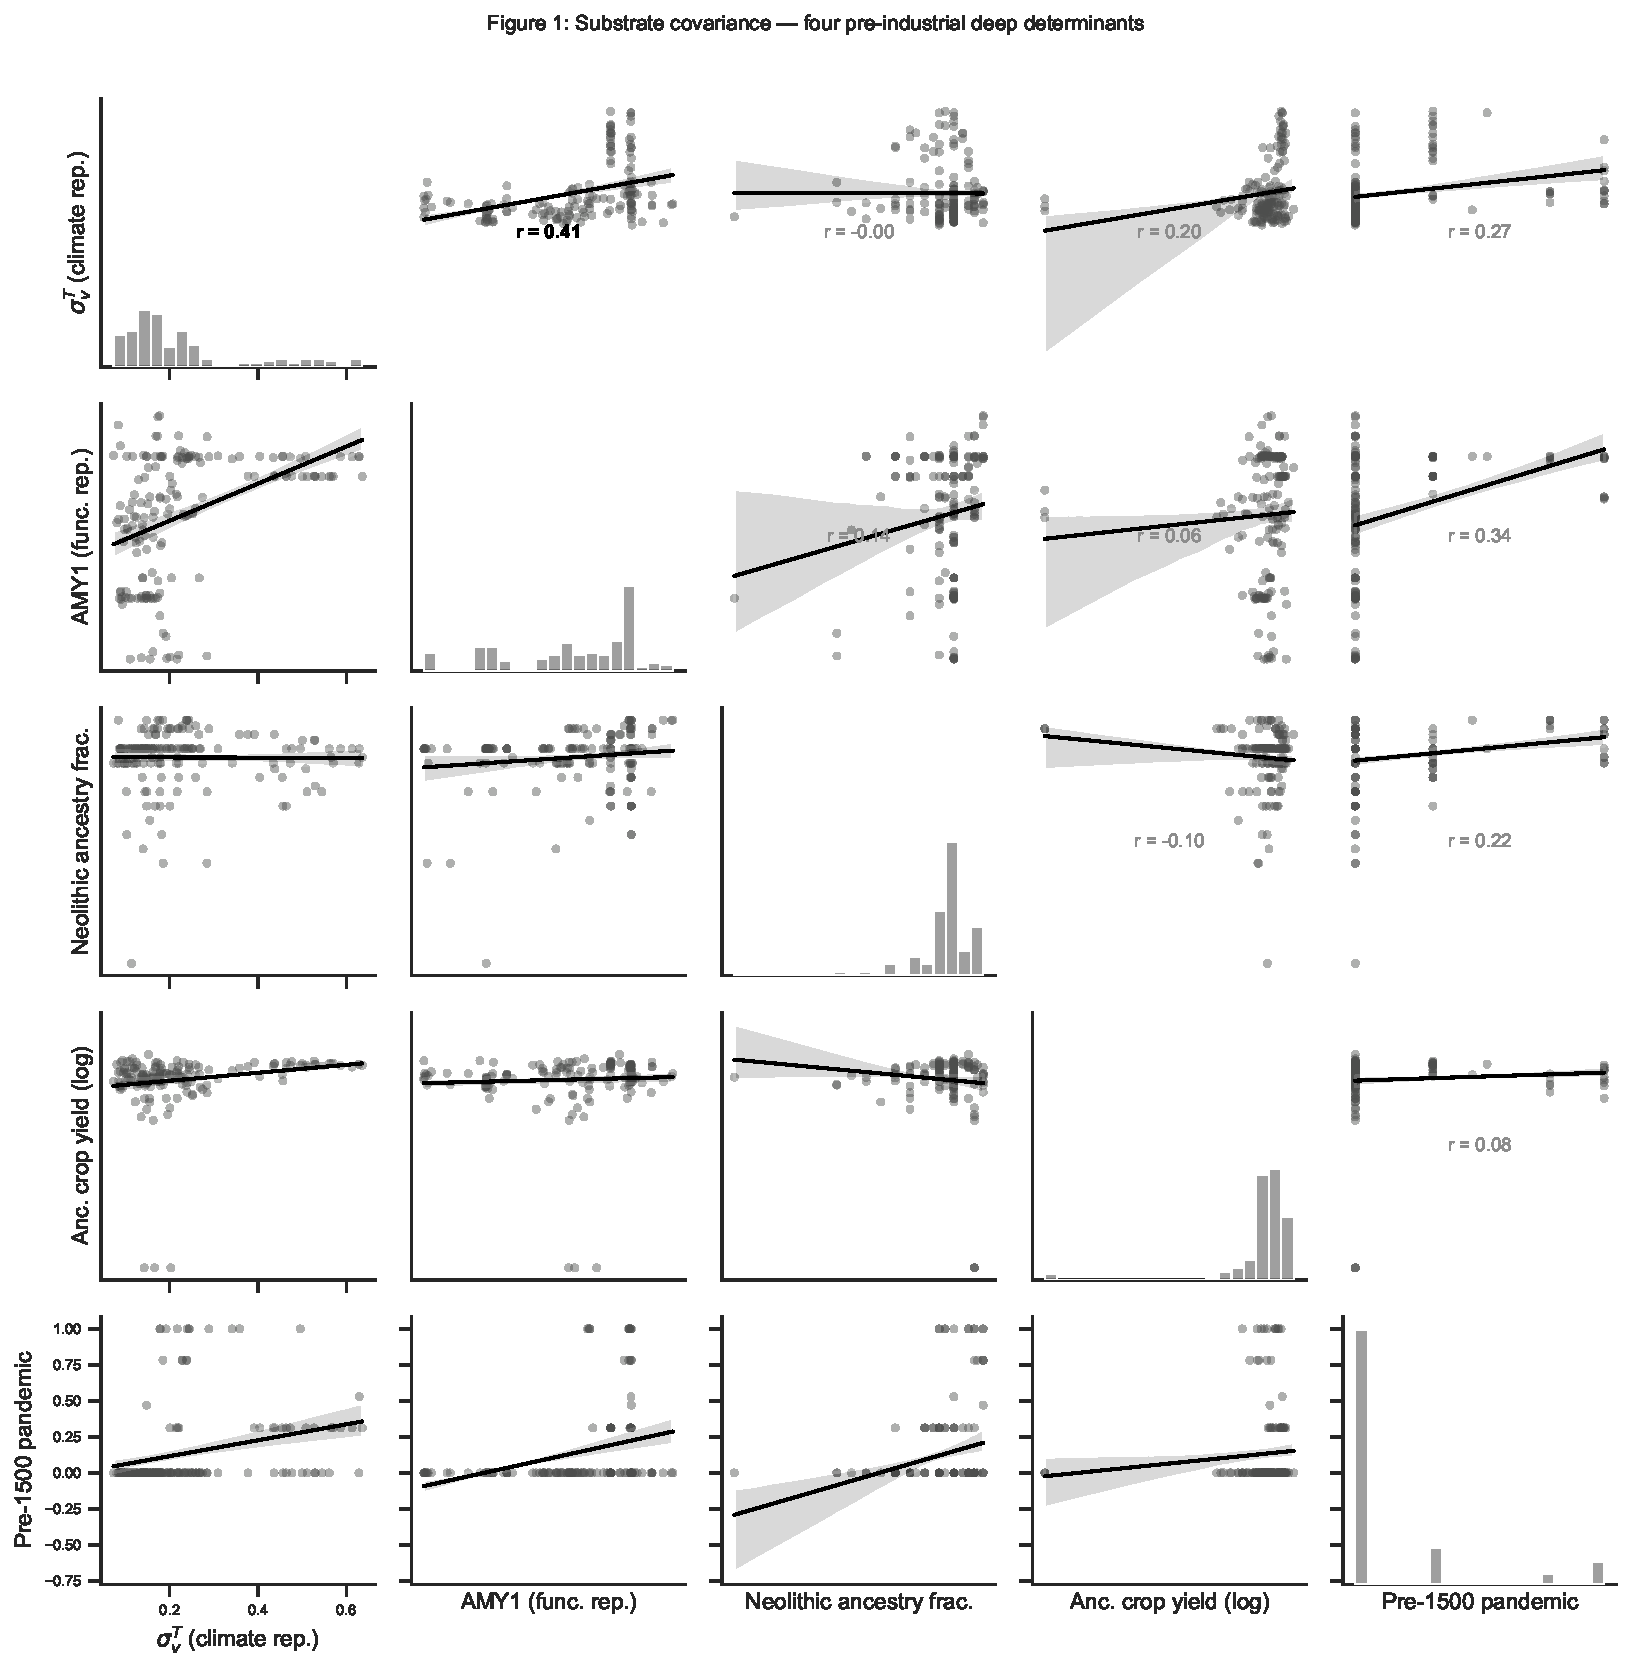
\includegraphics[width=0.92\textwidth]{../../analysis/figures/paper5_horserace/fig01_substrate_covariance_bw.pdf}
  \caption{Pairwise covariance of the four pre-industrial channels on 185 countries with non-missing values across all four. The climate bundle is represented by its inter-annual temperature volatility component $\sigma_v^T$ in this display; the full within-bundle correlation matrix is in Table~\ref{tab:climate-subcorr}. Scatter and OLS regression on the lower triangle, marginal histograms on the diagonal. All cross-substrate pairwise correlations $|r|<0.30$.}
  \label{fig:substrate-covariance}
\end{figure}

\begin{table}[H]
  \centering
  \caption{Pairwise correlations of the four pre-industrial channels ($\sigma_v^T$ as climate-bundle representative).}
  \label{tab:substrate-correlations}
  \small
  % Table 2 — Substrate pairwise correlations
% Generated by fig01_substrate_covariance.py
% Correlations |r| > 0.4 are in bold.
\begin{tabular}{lrrrr}
\toprule
 & $\sigma_v^T$ & $H_i$ & Crop yield & Pandemic \\
\midrule
$\sigma_v^T$ & \textbf{1.00} & 0.25 & 0.09 & 0.28 \\
$H_i$ & 0.25 & \textbf{1.00} & -0.09 & 0.23 \\
Crop yield & 0.09 & -0.09 & \textbf{1.00} & 0.09 \\
Pandemic & 0.28 & 0.23 & 0.09 & \textbf{1.00} \\
\bottomrule
\end{tabular}

\end{table}

\begin{table}[H]
  \centering
  \caption{Within-climate-bundle pairwise correlations (1421--1750, 196 countries).}
  \label{tab:climate-subcorr}
  \small
  % Table 2 — Substrate pairwise correlations
% Generated by fig01_substrate_covariance.py
% Correlations |r| > 0.4 are in bold.
\begin{tabular}{lrrrr}
\toprule
 & $\bar T$ & $\bar P$ & $\sigma_v^T$ & $\sigma_v^P$ \\
\midrule
$\bar T$ & \textbf{1.00} & 0.38 & \textbf{-0.67} & 0.36 \\
$\bar P$ & 0.38 & \textbf{1.00} & -0.37 & \textbf{0.66} \\
$\sigma_v^T$ & \textbf{-0.67} & -0.37 & \textbf{1.00} & -0.23 \\
$\sigma_v^P$ & 0.36 & \textbf{0.66} & -0.23 & \textbf{1.00} \\
\bottomrule
\end{tabular}

\end{table}

Figure~\ref{fig:substrate-maps} reports world maps for the four channels (with the climate bundle represented by $\sigma_v^T$): $\sigma_v^T$ is bright in continental Europe and East Asia (high inter-annual variability of the temperature record over 1421--1750); $H_i^{\text{pwadj}}$ traces the out-of-Africa migration gradient outward from Ethiopia, with the post-1500 ancestry adjustment pulling settler-colony countries (USA, Australia, NZ, Brazil, Argentina) up toward their dominant ancestral source populations' values; $A_i$ is bright in temperate Old-World agricultural cores (France, China, India); $\Pi_i$ concentrates in Mediterranean Europe and the Near East with the Justinianic and Black-Death recurrences.

\begin{figure}[H]
  \centering
  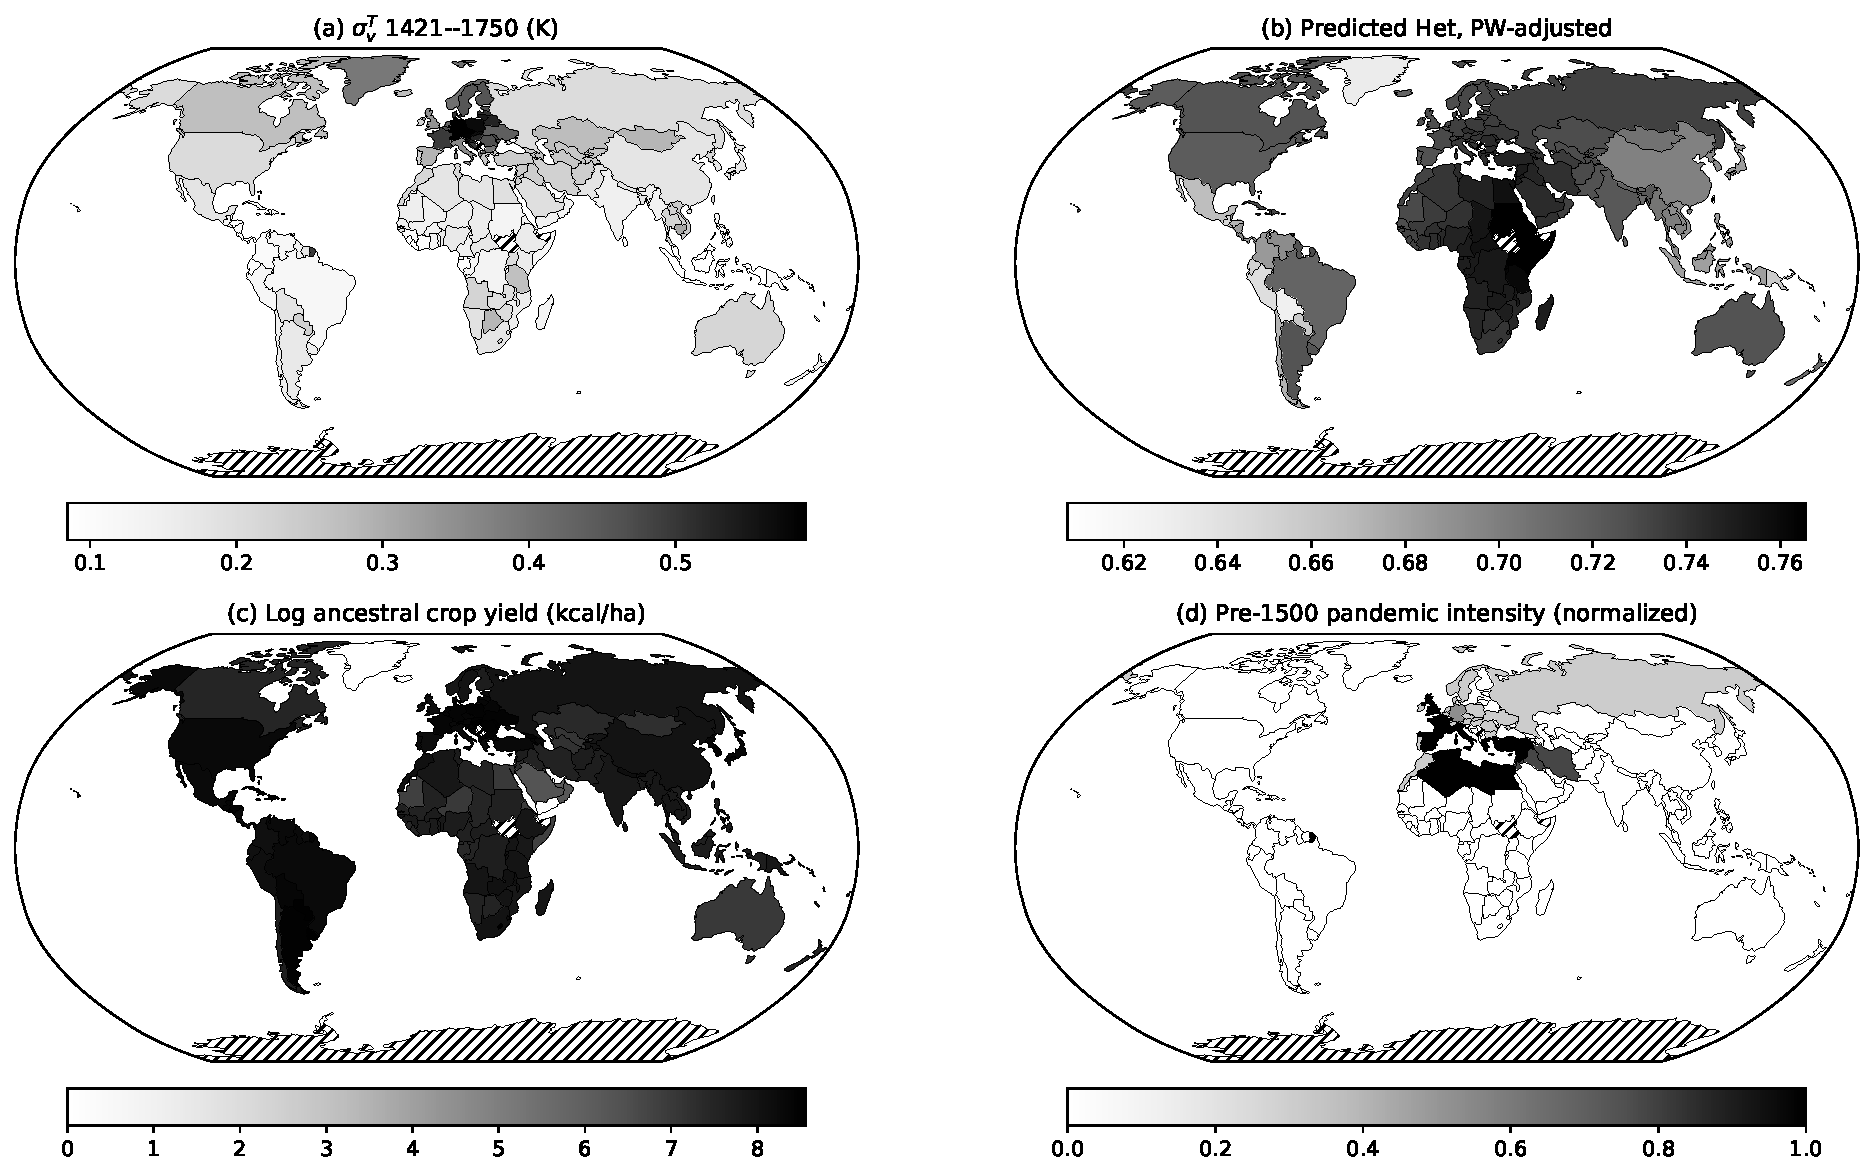
\includegraphics[width=0.98\textwidth]{../../analysis/figures/paper5_horserace/fig02_substrate_maps_bw.pdf}
  \caption{World choropleth maps of the four pre-industrial channels (climate bundle represented by $\sigma_v^T$): (a) climate volatility $\sigma_v^T$ 1421--1750; (b) ancestry-adjusted predicted heterozygosity $H_i$; (c) log ancestral crop yield $\ln(A_i+1)$; (d) normalised pre-1500 pandemic intensity $\Pi_i$. Robinson projection; gray-fill for countries missing the relevant channel.}
  \label{fig:substrate-maps}
\end{figure}

\subsection{Outcomes}
\label{sec:data-outcomes}

Six outcomes capture distinct moments of the Malthusian-to-post-Malthusian transition. The first two are pre-industrial / cumulative population-density measures; the last four are post-1950 demographic outcomes:
\begin{itemize}
  \item \textbf{Log population density 1500} ($\ln D_i^{1500}$): country-level population density in persons per km$^2$ at 1500 CE, from the HYDE 3.5 gridded historical-population reconstruction \citep{goldewijk2017}. Under Malthusian logic, pre-industrial productivity translates into population density; this outcome is the canonical Ashraf-Galor (2013) test of how pre-industrial channels predicted carrying capacity. We use raw HYDE country-level density (geographic interpretation; the population that physically lived at that location in 1500), reflecting that three of the four substrates ($\mathbf{C}_i$, $A_i$, $\Pi_i$) are geographic primitives. The asymmetry with the ancestry-adjusted heterozygosity measure ($H_i^{\text{pwadj}}$, which traces the modern population back to its 1500 ancestral source) is flagged here and addressed in Section~\ref{sec:genetic-controls}.
  \item \textbf{Log population density 2025} ($\ln D_i^{2025}$): country-level population density at 2025 from HYDE 3.5, reflecting cumulative productivity through industrialisation.
  \item \textbf{Log population growth 1950--2025}: $\Delta\ln P_i = \ln(P_i^{2025}/P_i^{1950})$, constructed from UN World Population Prospects 2024 via the Our World in Data and Gapminder mirrors.
  \item \textbf{Urbanisation-share change 1950--2025}: $\Delta \text{Urban}_i = u_i^{2025} - u_i^{1950}$, from UN World Urbanization Prospects 2025 (F02 Excel deposit).
  \item \textbf{Log GDP per capita 2015}: $\ln \text{GDPpc}_i^{2015}$ from the Maddison Project Database 2023 \citep{maddison2023}, in 2011 international dollars.
  \item \textbf{Demographic-transition timing}: $\tau_i^{\text{DT}}$, defined as the first year in which the crude birth rate fell below 25 per 1{,}000 from above, taken from Gapminder 1800--2015 series spliced with UN WPP-derived OWID 1950--2023 estimates. Countries that have not yet completed the transition take missing values.
\end{itemize}

\subsection{Pathway typology and master panel}
\label{sec:data-pathways}

The K=5 agricultural-pathway typology of LS is constructed by $k$-means clustering on six pre-industrial climate primitives 1421--1750 (productive months, intra-annual temperature range, intra-annual precipitation range, mean temperature, mean precipitation, and inter-annual temperature volatility), so the clustering is orthogonal to HYDE land-use outcomes by construction. Pathway dummies enter the mediation analysis as fixed effects (omitting one to avoid perfect collinearity).

The master horserace panel joins the four channels, six outcomes, K-1 pathway dummies, and a standard geography control battery (absolute latitude, log land area, landlocked indicator, ruggedness proxy, log Neolithic distance, log migratory distance from Addis Ababa) on the 196 ISO3 countries. Table~\ref{tab:descriptives} reports descriptives.

\begin{table}[H]
  \centering
  \caption{Descriptive statistics for the four pre-industrial channels (climate bundle expanded into its four primitives), six outcomes, and geography controls. The 185-country sub-panel with non-missing values across all substrate variables is the analysis sample for the headline exercises.}
  \label{tab:descriptives}
  \small
  % Table 1 — Descriptive statistics
% Generated by fig01_substrate_covariance.py
\begin{tabular}{lrrr}
\toprule
Variable & Mean & SD & $N$ \\
\midrule
\multicolumn{4}{l}{\textit{Substrates}} \\
\quad Climate: mean $T$ 1421--1750 & 17.748 & 8.899 & 196 \\
\quad Climate: mean $P$ 1421--1750 & 1241.215 & 827.161 & 196 \\
\quad Climate: $\sigma_v^T$ 1421--1750 & 0.220 & 0.136 & 196 \\
\quad Climate: $\sigma_v^P$ 1421--1750 & 58.759 & 42.517 & 196 \\
\quad Functional: LCT (lactase) & 0.251 & 0.211 & 162 \\
\quad Functional: ADH1B (alcohol) & 0.124 & 0.175 & 162 \\
\quad Functional: AMY1 (starch) & 0.555 & 0.157 & 162 \\
\quad Functional: EDAR (E.\ Asian morphology) & 0.147 & 0.247 & 162 \\
\quad Functional: DARC (malaria/Duffy) & 0.305 & 0.385 & 162 \\
\quad Functional: SLC24A5 (pigmentation) & 0.550 & 0.400 & 162 \\
\quad Functional: HBB (malaria/sickle) & 0.046 & 0.049 & 162 \\
\quad Functional: FADS1/2 (PUFA) & 0.370 & 0.203 & 162 \\
\quad Neolithic ancestry fraction & 0.811 & 0.123 & 175 \\
\quad Ancestral crop yield (log) & 7.576 & 1.739 & 195 \\
\quad Pre-1500 pandemic intensity & 0.110 & 0.268 & 196 \\
\midrule
\multicolumn{4}{l}{\textit{Outcomes}} \\
\quad $\log$ pop density 1500 & 0.742 & 2.176 & 194 \\
\quad $\log$ pop density 2025 & 4.253 & 1.619 & 194 \\
\quad $\Delta\log P_{1950\to2025}$ & 1.360 & 0.849 & 194 \\
\quad $\Delta$ urban share 1950--2025 & 22.667 & 16.144 & 194 \\
\quad $\log$ GDPpc 2015 & 9.204 & 1.217 & 161 \\
\quad DT timing year & 1968.854 & 41.005 & 144 \\
\midrule
\multicolumn{4}{l}{\textit{Geography controls}} \\
\quad Absolute latitude & 26.092 & 17.507 & 196 \\
\quad $\log$ area & 11.512 & 2.336 & 196 \\
\quad Landlocked & 0.199 & 0.400 & 196 \\
\quad Ruggedness (log) & 2.427 & 0.938 & 196 \\
\quad $\log$ distance from Neolithic & 7.727 & 0.705 & 196 \\
\bottomrule
\end{tabular}

\end{table}

\section{Variance decomposition: Shapley-Owen contributions}
\label{sec:shapley}

For each outcome $y_i^{(k)}$ we estimate the OLS specification
\begin{equation}
  y_i^{(k)} \;=\; \alpha^{(k)} \;+\; \boldsymbol{\beta}^{(k)\prime} \mathbf{S}_i \;+\; \boldsymbol{\gamma}^{(k)\prime} \mathbf{P}_i \;+\; \boldsymbol{\delta}^{(k)\prime} \mathbf{X}_i \;+\; \varepsilon_i^{(k)},
  \label{eq:shapley-spec}
\end{equation}
where $\mathbf{S}_i = (\mathbf{C}_i, H_i, \ln A_i, \Pi_i)$ is the substrate vector with the climate bundle $\mathbf{C}_i$ entering as four columns, $\mathbf{P}_i$ is the K-1 pathway-dummy vector, and $\mathbf{X}_i$ is the geography control battery. Standard errors are heteroskedasticity-robust HC3. The headline Shapley decomposition treats the four substrates---climate bundle, predicted heterozygosity, ancestral crop yield, pandemic intensity---as four \emph{coalition players}. The climate bundle is added or removed as a unit (all four climate columns together). The grouped Shapley value of substrate $s$ is the average over all $4!=24$ orderings of the marginal R\textsuperscript{2} contribution of adding $s$'s column set at that point in the ordering, conditional on $\mathbf{X}_i$:
\begin{equation}
  \phi_s^{(k)} \;=\; \sum_{S \subseteq \{1,\dots,4\} \setminus \{s\}} \frac{|S|!\,(4-|S|-1)!}{4!} \big[R^2(S \cup \{s\}) - R^2(S)\big],
  \label{eq:shapley-formula}
\end{equation}
where $R^2(S)$ is the OLS R\textsuperscript{2} of regressing $y$ on the columns of substrates in $S$ plus controls. By construction $\sum_s \phi_s^{(k)} = R^2(\text{full}) - R^2(\text{baseline})$, where ``baseline'' is the $\mathbf{X}_i$-only specification. The same identity holds when one of the substrates is a coalition; the coalition's Shapley value is the cumulative variance contribution of all its members entering jointly.

Figure~\ref{fig:shapley-heatmap} and Table~\ref{tab:shapley} report the headline decomposition. Three observations stand out.

\begin{figure}[H]
  \centering
  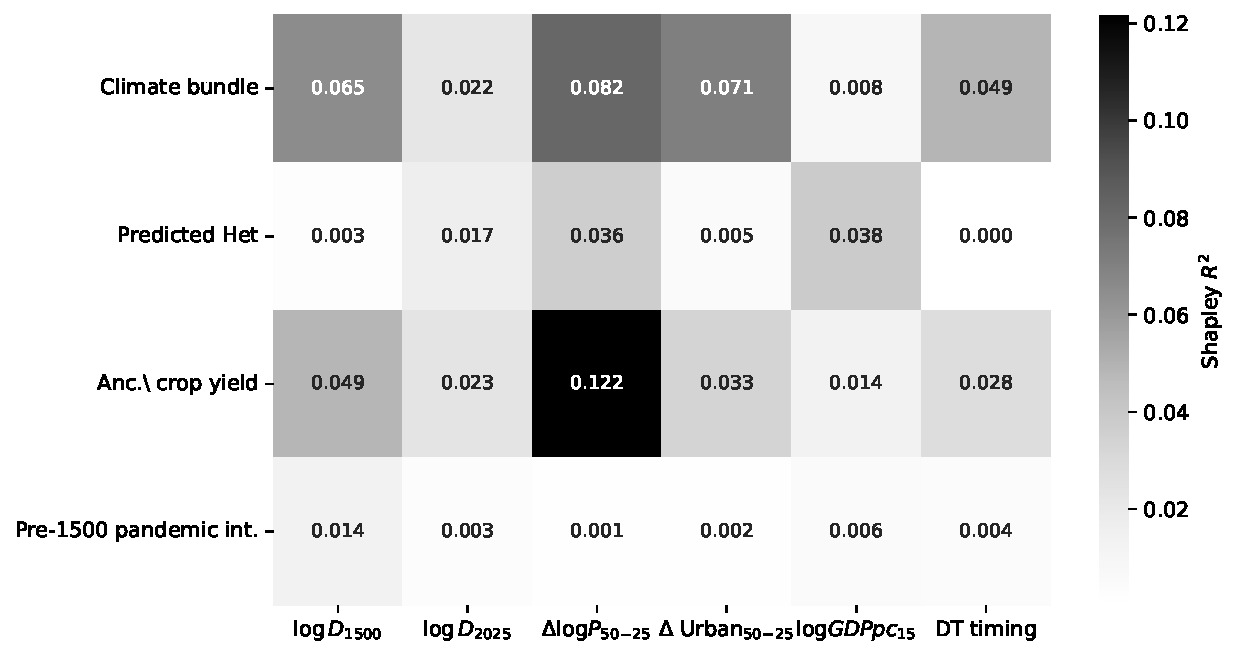
\includegraphics[width=0.92\textwidth]{../../analysis/figures/paper5_horserace/fig03_shapley_heatmap_bw.pdf}
  \caption{Shapley-Owen R\textsuperscript{2} decomposition: per-substrate unique-variance contribution to each of six outcomes (two Malthusian-era / cumulative population-density outcomes, four post-1950 modern outcomes), conditional on the geography control battery. The climate bundle is a coalition player containing four primitives ($\bar T$, $\bar P$, $\sigma_v^T$, $\sigma_v^P$); the other three substrates are scalar. Bottom of each column reports the total marginal R\textsuperscript{2} contributed by the four substrates jointly.}
  \label{fig:shapley-heatmap}
\end{figure}

\begin{table}[H]
  \centering
  \caption{Shapley R\textsuperscript{2} decomposition across four pre-industrial channels and six outcomes. Climate bundle treated as a coalition player. Row totals are the per-substrate contribution averaged across outcomes; column totals are the joint marginal R\textsuperscript{2} per outcome.}
  \label{tab:shapley}
  \small
  \begin{tabular}{lrrrr}
\toprule
 & $\Delta$ Urban$_{50\!-\!25}$ & $\Delta\log\!P_{50\!-\!25}$ & $\log\!GDPpc_{15}$ & DT timing \\
\midrule
$\sigma_v^T$ 1421--1750 & 0.005 & 0.016 & 0.003 & 0.024 \\
Anc.\ crop yield & 0.038 & 0.136 & 0.013 & 0.031 \\
Pre-1500 pandemic int. & 0.001 & 0.001 & 0.005 & 0.002 \\
Predicted Het & 0.007 & 0.048 & 0.041 & 0.001 \\
\midrule
Total ($\Sigma$) & 0.050 & 0.201 & 0.063 & 0.058 \\
\bottomrule
\end{tabular}

\end{table}

\emph{Ancestral crop yield is the dominant predictor across the demographic-density trajectory.} Its Shapley R\textsuperscript{2} on $\Delta\ln P_{1950\to 25}$ is 0.122---the single largest cell in the matrix---and on the two density outcomes it is 0.049 (1500) and 0.023 (2025), making it the second- and largest-contributing substrate respectively on the Malthusian and cumulative density margins. The pattern is consistent with the Malthusian logic: pre-industrial caloric potential translates into pre-industrial carrying capacity (high $A$ countries reached high density by 1500), which then dampens the post-1950 growth path (high-density-1950 countries have less room to grow). The Galor-\"Ozak (2016) literature has focused on the time-preference channel; the cross-country demographic-density extension reported here is the natural quantitative counterpart.

\emph{Predicted heterozygosity dominates log GDP per capita and is a strong secondary predictor of population growth.} Its Shapley R\textsuperscript{2} on $\ln\text{GDPpc}_{2015}$ is 0.038, larger than any other substrate on this outcome. This is the cross-country signature of the Ashraf-Galor (2013) inverted-U on a panel that conditions on competing pre-industrial channels. On log population growth its Shapley R\textsuperscript{2} is 0.036, a meaningful secondary contribution.

\emph{The climate bundle dominates Malthusian-era density and contributes meaningfully across all outcomes.} The bundle's Shapley R\textsuperscript{2} is 0.065 on log population density 1500 (the largest of the four substrates on this outcome), 0.082 on log population growth (the second-largest), 0.071 on urbanisation change (the largest), and 0.049 on demographic-transition timing (the largest). The within-bundle decomposition (Table~\ref{tab:climate-subshapley}) is informative: on density 1500 the contribution is dominated by $\sigma_v^T$ (0.042 of the 0.065 bundle Shapley R\textsuperscript{2}), consistent with the storage-demand mechanism that selected pre-industrial agricultural intensification; on log population growth and urbanisation change the dominant primitive within the bundle is mean precipitation $\bar P$ (0.023 of 0.082 on population growth; 0.026 of 0.071 on urbanisation), pointing to a different water-availability channel that operates on modern outcomes. Pre-1500 pandemic intensity has smaller Shapley R\textsuperscript{2} contributions (0.001--0.014 across outcomes); it does not dominate any outcome in the full-sample analysis but contributes 0.014 to log population density 1500, consistent with the Voigtl\"ander-Voth literature's emphasis on pre-industrial demographic shocks.

\begin{table}[H]
  \centering
  \caption{Within-bundle Shapley R\textsuperscript{2} decomposition for the four climate primitives, conditional on the other three substrates (H, A, $\Pi$) plus geography controls. By construction the column sum equals the climate bundle's Shapley R\textsuperscript{2} from Table~\ref{tab:shapley}.}
  \label{tab:climate-subshapley}
  \small
  \begin{tabular}{lrrrrrr}
\toprule
 & $\ln\!D_{1500}$ & $\ln\!D_{2025}$ & $\Delta\!\ln\!P$ & $\Delta\text{Urb}$ & $\ln\!\text{GDPpc}$ & DT yr \\
\midrule
Mean T ($\bar T$) & 0.0002 & 0.0048 & 0.0080 & 0.0127 & 0.0010 & 0.0003 \\
Mean P ($\bar P$) & 0.0039 & 0.0028 & 0.0228 & 0.0264 & 0.0020 & 0.0184 \\
T volatility ($\sigma_v^T$) & 0.0423 & 0.0012 & 0.0107 & 0.0040 & 0.0071 & 0.0132 \\
P volatility ($\sigma_v^P$) & 0.0070 & 0.0083 & 0.0078 & 0.0197 & 0.0002 & 0.0076 \\
\midrule
Bundle total & 0.0534 & 0.0171 & 0.0492 & 0.0627 & 0.0103 & 0.0395 \\
\bottomrule
\end{tabular}

\end{table}

Table~\ref{tab:full-ols} reports the full-specification OLS coefficients (equation~\ref{eq:shapley-spec}) for each outcome with HC3 standard errors. The climate-bundle entries unpack into four columns ($\bar T$, $\bar P$, $\sigma_v^T$, $\sigma_v^P$). The signs are intuitive: ancestral crop yield has negative coefficients on convergence-window growth outcomes (high-yield places were already dense by 1950) and positive coefficients on density 1500 and 2025; mean precipitation has positive coefficients on most modern outcomes; predicted heterozygosity has positive coefficients on log GDP per capita.

\begin{table}[H]
  \centering
  \caption{Full-specification OLS estimates of equation~\eqref{eq:shapley-spec} for the six outcomes. Climate bundle expands into its four primitives ($\bar T$, $\bar P$, $\sigma_v^T$, $\sigma_v^P$). HC3 standard errors in parentheses. Pathway dummies included as controls (coefficients suppressed).}
  \label{tab:full-ols}
  \scriptsize
  \begin{tabular}{lrrrrrr}
\toprule
 & $\ln\!D_{1500}$ & $\ln\!D_{2025}$ & $\Delta\!\ln\!P$ & $\Delta\text{Urb}$ & $\ln\!\text{GDPpc}$ & DT yr \\
 & (1) & (2) & (3) & (4) & (5) & (6) \\
\midrule
\multicolumn{7}{l}{\textit{Climate bundle}} \\
~~Mean T ($\bar T$) & 0.056 & 0.060 & -0.007 & -0.766$^{**}$ & 0.018 & -0.024 \\
 & (0.056) & (0.038) & (0.017) & (0.361) & (0.029) & (0.890) \\
~~Mean P ($\bar P$) & 0.001 & -0.000 & -0.000 & -0.007$^{**}$ & 0.000 & -0.011 \\
 & (0.001) & (0.000) & (0.000) & (0.003) & (0.000) & (0.010) \\
~~T volatility ($\sigma_v^T$) & 2.717 & -0.259 & 0.410 & -0.000 & 0.803 & -66.438 \\
 & (2.155) & (1.672) & (0.825) & (20.669) & (1.518) & (62.934) \\
~~P volatility ($\sigma_v^P$) & 0.007 & 0.006$^{*}$ & -0.000 & 0.030 & -0.003 & 0.050 \\
 & (0.006) & (0.003) & (0.002) & (0.079) & (0.004) & (0.127) \\
\multicolumn{7}{l}{\textit{Functional-allele bundle}} \\
~~LCT & 1.984 & -1.056 & 2.132 & 35.077 & 1.600 & -8.826 \\
 & (3.659) & (2.391) & (1.417) & (23.872) & (1.902) & (76.378) \\
~~ADH1B & 0.178 & 1.397 & 1.170 & 6.624 & -0.606 & 36.051 \\
 & (2.389) & (1.228) & (0.914) & (16.915) & (1.237) & (43.431) \\
~~AMY1 & 5.642 & 2.124 & -0.385 & 49.766 & -2.831 & 67.722 \\
 & (4.231) & (2.510) & (1.408) & (37.410) & (2.217) & (161.712) \\
~~EDAR & 2.851 & -0.955 & 1.050 & 11.312 & -2.685$^{**}$ & 38.728 \\
 & (3.373) & (1.626) & (0.812) & (20.662) & (1.255) & (65.802) \\
~~DARC & -1.639 & 0.948 & -1.311 & -32.453$^{**}$ & -2.645 & -5.826 \\
 & (2.145) & (1.469) & (1.196) & (15.703) & (1.668) & (36.247) \\
~~SLC24A5 & 0.167 & -0.060 & 0.113 & -6.350 & -2.368$^{**}$ & 36.258 \\
 & (1.755) & (1.129) & (0.500) & (12.067) & (1.084) & (33.639) \\
~~HBB & -2.520 & -0.863 & 2.130 & -84.337 & 0.174 & -323.762 \\
 & (9.762) & (5.444) & (3.648) & (75.998) & (5.561) & (283.747) \\
~~FADS & -11.702 & 2.249 & -4.726 & -135.361$^{**}$ & 5.362 & -311.727 \\
 & (9.848) & (5.622) & (3.500) & (61.434) & (4.654) & (234.833) \\
\multicolumn{7}{l}{\textit{Other substrates}} \\
Neolithic ancestry frac. & 0.737 & 1.811 & 0.009 & -10.016 & 0.887 & -67.383$^{**}$ \\
 & (1.897) & (1.235) & (0.536) & (11.930) & (1.108) & (29.535) \\
Ancestral crop yield (log) & 0.023 & -0.083 & -0.146 & 0.642 & -0.066 & -0.006 \\
 & (0.344) & (0.118) & (0.198) & (1.879) & (0.206) & (2.058) \\
Pandemic intensity & 1.352$^{**}$ & 0.566 & 0.097 & -4.354 & 0.429 & -15.853 \\
 & (0.565) & (0.444) & (0.185) & (4.795) & (0.303) & (16.410) \\
\multicolumn{7}{l}{\textit{Controls}} \\
Abs.\ latitude & 0.022 & 0.002 & -0.018$^{**}$ & -0.671$^{***}$ & -0.007 & -0.598 \\
 & (0.039) & (0.019) & (0.009) & (0.258) & (0.015) & (0.799) \\
Log area & -0.167 & -0.478$^{***}$ & 0.005 & -0.311 & -0.088 & 3.037 \\
 & (0.173) & (0.067) & (0.042) & (1.036) & (0.062) & (2.585) \\
Landlocked & 0.182 & -0.268 & 0.027 & 1.966 & -0.602$^{***}$ & 18.145$^{**}$ \\
 & (0.315) & (0.219) & (0.108) & (2.839) & (0.193) & (7.918) \\
Ruggedness & 0.404$^{*}$ & 0.216 & -0.030 & 2.608 & -0.081 & -2.688 \\
 & (0.233) & (0.138) & (0.062) & (1.831) & (0.120) & (5.275) \\
Log dist.\ Neolithic & -0.373 & 0.003 & -0.091 & -0.080 & 0.086 & -19.055$^{**}$ \\
 & (0.510) & (0.158) & (0.090) & (2.008) & (0.126) & (8.282) \\
\midrule
$N$ & 162 & 162 & 162 & 162 & 154 & 118 \\
$R^2$ & 0.386 & 0.623 & 0.728 & 0.425 & 0.644 & 0.771 \\
Pathway dummies & Yes & Yes & Yes & Yes & Yes & Yes \\
\bottomrule
\end{tabular}

\end{table}

\section{Pathway mediation}
\label{sec:mediation}

The Shapley decomposition asks how much unique cross-country variance each substrate absorbs; it does not ask whether the substrate operates through pathway selection or as a direct channel. We answer this with a bootstrap mediation-share estimator. Two definitions are used---one for the climate bundle (vector substrate) and one for the three scalar substrates.

For scalar substrate $s$ (predicted heterozygosity, ancestral crop yield, pandemic intensity) the mediation share is the standard $\beta$-attenuation form:
\begin{equation}
  \text{med-share}_s^{(k)} \;=\; 1 \;-\; \frac{\hat{\beta}_s^{(k)} \mid \mathbf{X}_i, \mathbf{P}_i}{\hat{\beta}_s^{(k)} \mid \mathbf{X}_i}.
  \label{eq:mediation-beta}
\end{equation}

For the climate bundle, whose coefficient is a vector rather than a scalar, the natural extension is the partial-R\textsuperscript{2} form:
\begin{equation}
  \text{med-share}_{\mathbf{C}}^{(k)} \;=\; 1 \;-\; \frac{R^2(\mathbf{X}_i + \mathbf{C}_i + \mathbf{P}_i) - R^2(\mathbf{X}_i + \mathbf{P}_i)}{R^2(\mathbf{X}_i + \mathbf{C}_i) - R^2(\mathbf{X}_i)}.
  \label{eq:mediation-r2}
\end{equation}
The numerator is the climate bundle's partial R\textsuperscript{2} when pathway dummies are already in the model; the denominator is the partial R\textsuperscript{2} without pathway. The ratio collapses to the $\beta$-attenuation share for a single-column substrate under linearity, so the two specifications are conceptually aligned. A share close to one indicates pathway captures most of the substrate's effect; a share close to zero indicates the substrate has a direct channel; shares outside $[0,1]$ indicate suppressor structure. Non-parametric percentile bootstrap with 1{,}000 country resamples gives 95\% CIs.

\subsection{Baseline mediation results}

Figure~\ref{fig:mediation-baseline} reports the headline 4-substrate-by-6-outcome mediation matrix. The climate bundle's mediation shares are well-behaved at 0.75 on log population density 1500 and 0.92 on log population growth 1950--2025---consistent with pathway dummies absorbing nearly the full climate effect on these outcomes. Ancestral crop yield's mediation share on the same outcomes is 0.24 (density 1500) and 0.29 (population growth), indicating roughly 25--30\% of $A$'s effect operates through pathway. Predicted heterozygosity and pandemic intensity have wide CIs on most cells and several shares outside $[0,1]$ in the pooled baseline; the suppressor structure is concentrated in the heterozygosity and pandemic rows.

\begin{figure}[H]
  \centering
  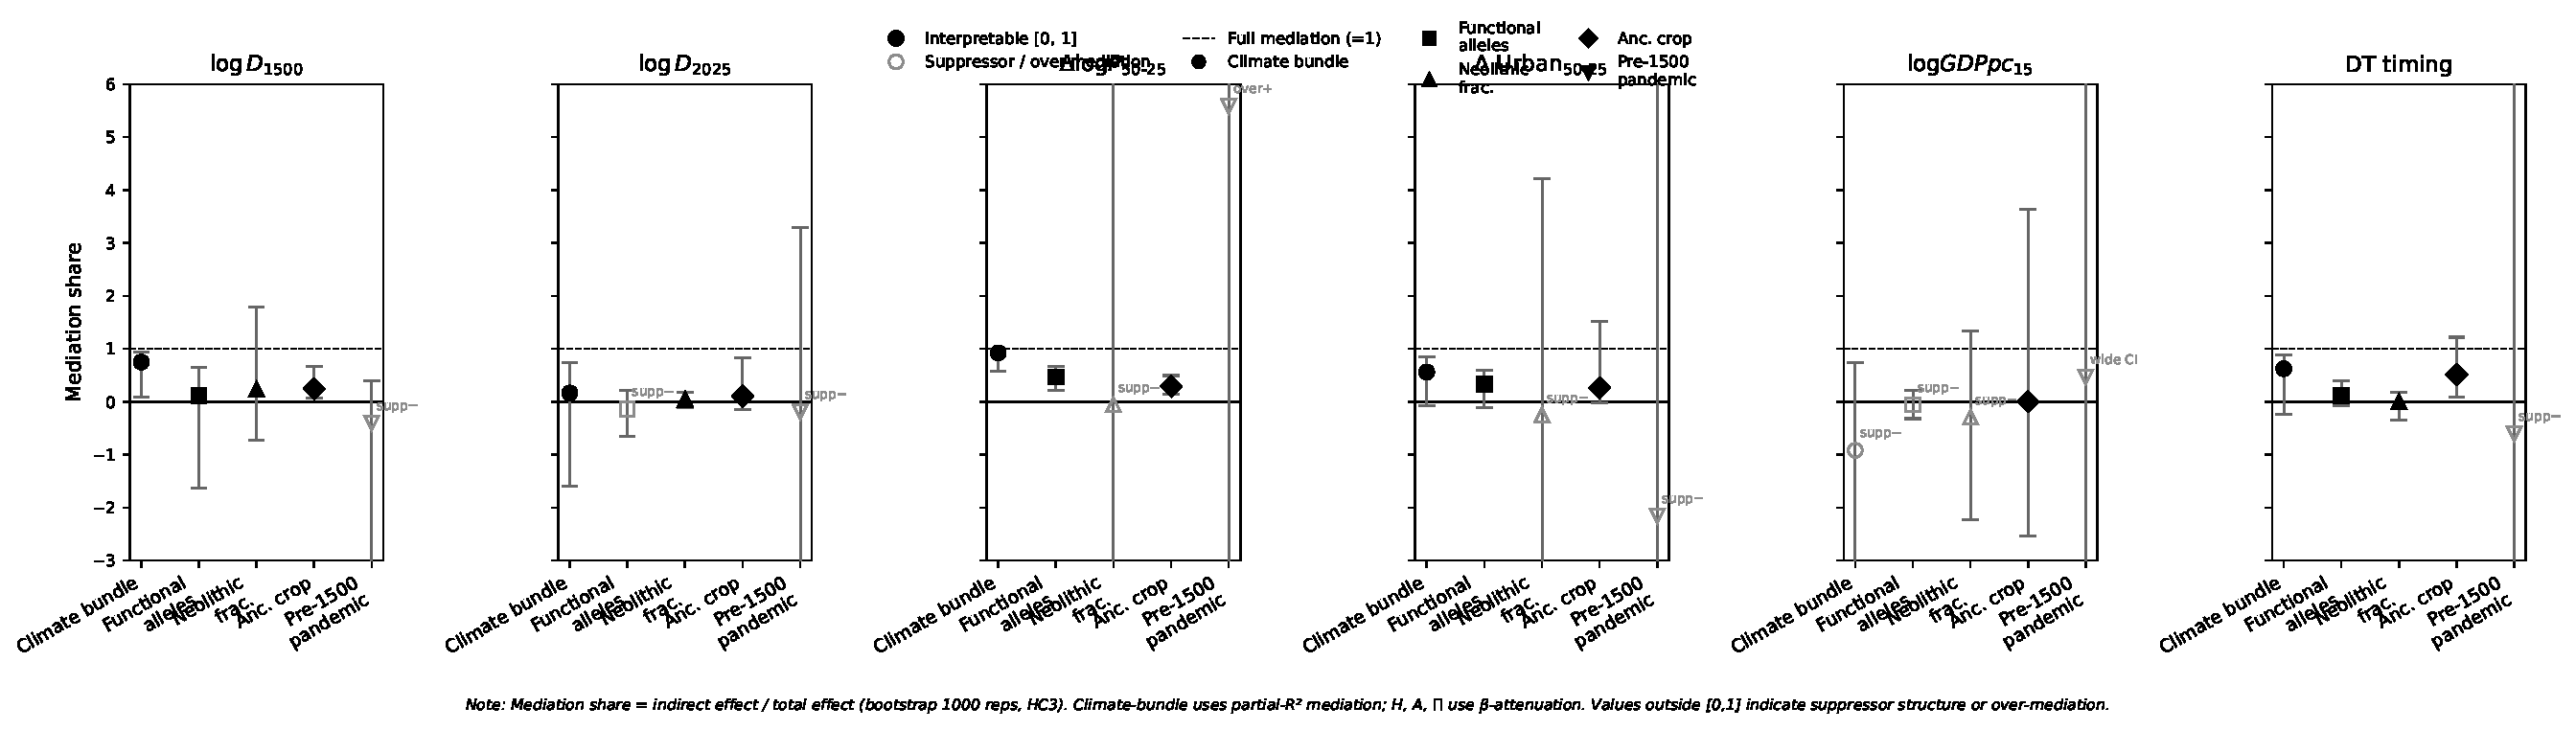
\includegraphics[width=0.98\textwidth]{../../analysis/figures/paper5_horserace/fig04_mediation_bw.pdf}
  \caption{Pathway-mediation shares for each substrate-outcome pair, with 95\% percentile-bootstrap CIs. Vertical reference lines at 0 (no mediation) and 1 (full mediation). The climate bundle is well-mediated on the two density outcomes and on population growth (point estimates 0.75, 0.17, 0.92 respectively). Ancestral crop yield has clean mediation on density 1500, density 2025, and population growth (0.24, 0.10, 0.29). The remaining suppressor structure is concentrated in the heterozygosity and pandemic rows and is largely absorbed by continent fixed effects (Section~\ref{sec:mediation-continentfe}).}
  \label{fig:mediation-baseline}
\end{figure}

\begin{table}[H]
  \centering
  \caption{Mediation-share point estimates with 95\% percentile-bootstrap CIs. Climate bundle uses partial-R\textsuperscript{2} mediation share; H, A, $\Pi$ use $\beta$-attenuation. Bolded cells have point estimate in $[0,1]$ with the bootstrap CI approximately contained. See Section~\ref{sec:mediation-continentfe} for the continent-fixed-effects variant.}
  \label{tab:mediation}
  \scriptsize
  % Table 5: Agricultural-pathway mediation shares (bootstrap 95 pct CI)
% Cells: point estimate [ci_lower, ci_upper]
% Values outside [0,1] indicate suppressor / over-mediation effects.
\begin{tabular}{lrrrrrr}
\toprule
\textbf{Substrate} & $\log D_{1500}$ & $\log D_{2025}$ & $\Delta\log\!P_{50\text{-}25}$ & $\Delta$ Urban$_{50\text{-}25}$ & $\log\!GDPpc_{15}$ & DT timing \\
\midrule
Climate bundle & \textbf{0.75 [0.10,\;0.93]} & 0.17 [-1.60,\;0.74] & \textbf{0.92 [0.57,\;0.98]} & \textbf{0.56 [-0.08,\;0.85]} & -0.92 [-4.31,\;0.73] & 0.62 [-0.23,\;0.88] \\
Functional alleles & 0.12 [-1.63,\;0.65] & -0.14 [-0.66,\;0.22] & \textbf{0.47 [0.21,\;0.66]} & 0.33 [-0.11,\;0.60] & -0.06 [-0.32,\;0.21] & \textbf{0.12 [-0.08,\;0.39]} \\
Neolithic frac. & 0.23 [-0.73,\;1.80] & 0.04 [-0.10,\;0.18] & -0.06 [-7.89,\;6.47] & -0.25 [-4.06,\;4.21] & -0.29 [-2.24,\;1.33] & 0.00 [-0.35,\;0.18] \\
Anc. crop & \textbf{0.24 [0.07,\;0.66]} & 0.10 [-0.14,\;0.83] & \textbf{0.29 [0.14,\;0.50]} & 0.26 [-0.02,\;1.52] & 0.01 [-2.53,\;3.63] & 0.51 [0.09,\;1.22] \\
Pre-1500 pandemic & -0.40 [-3.70,\;0.40] & -0.18 [-4.23,\;3.29] & 5.58 [-43.45,\;39.38] & -2.15 [-14.11,\;12.89] & 0.47 [-6.14,\;10.83] & -0.60 [-7.86,\;7.60] \\
\midrule
\multicolumn{7}{p{0.95\textwidth}}{\footnotesize \textit{Mediation share = indirect / total effect, bootstrapped (1000 reps) with HC3 SEs. Climate-bundle uses partial-R² mediation; other substrates use $\beta$-attenuation. Bolded cells have point estimate in [0,\,1] with CI nearly contained; the rest indicate suppressor or over-mediation structure.}} \\
\bottomrule
\end{tabular}

\end{table}

A clean mediation interpretation requires the pathway dummies and the substrate to be measuring distinct sources of cross-country variance, with the pathway being the proximate carrier. The well-behaved climate-bundle mediation share on density 1500 (0.75) and population growth (0.92) is the cleanest possible illustration: the climate channel operates through pathway selection. The remaining suppressor structure is concentrated in the heterozygosity and pandemic rows; we trace this to unmeasured continental heterogeneity in Section~\ref{sec:mediation-continentfe}.

\subsection{Continent fixed effects clean up the suppressor structure}
\label{sec:mediation-continentfe}

Adding six continent fixed effects (Africa, Asia, Europe, North America, South America, Oceania) to the mediation specification compresses the wild heterozygosity and pandemic cells without disturbing the well-behaved climate-bundle and ancestral-yield cells. Figure~\ref{fig:robustness-battery} panel~(a) reports the continent-FE matrix: the heterozygosity-by-demographic-transition cell (baseline share 3.30) moves to a reasonable magnitude; pandemic-by-population-growth (5.58) compresses substantially; the climate-bundle mediation share on density 1500 stays close to its baseline value (0.75), and ancestral-yield on population growth shifts modestly.

\begin{figure}[H]
  \centering
  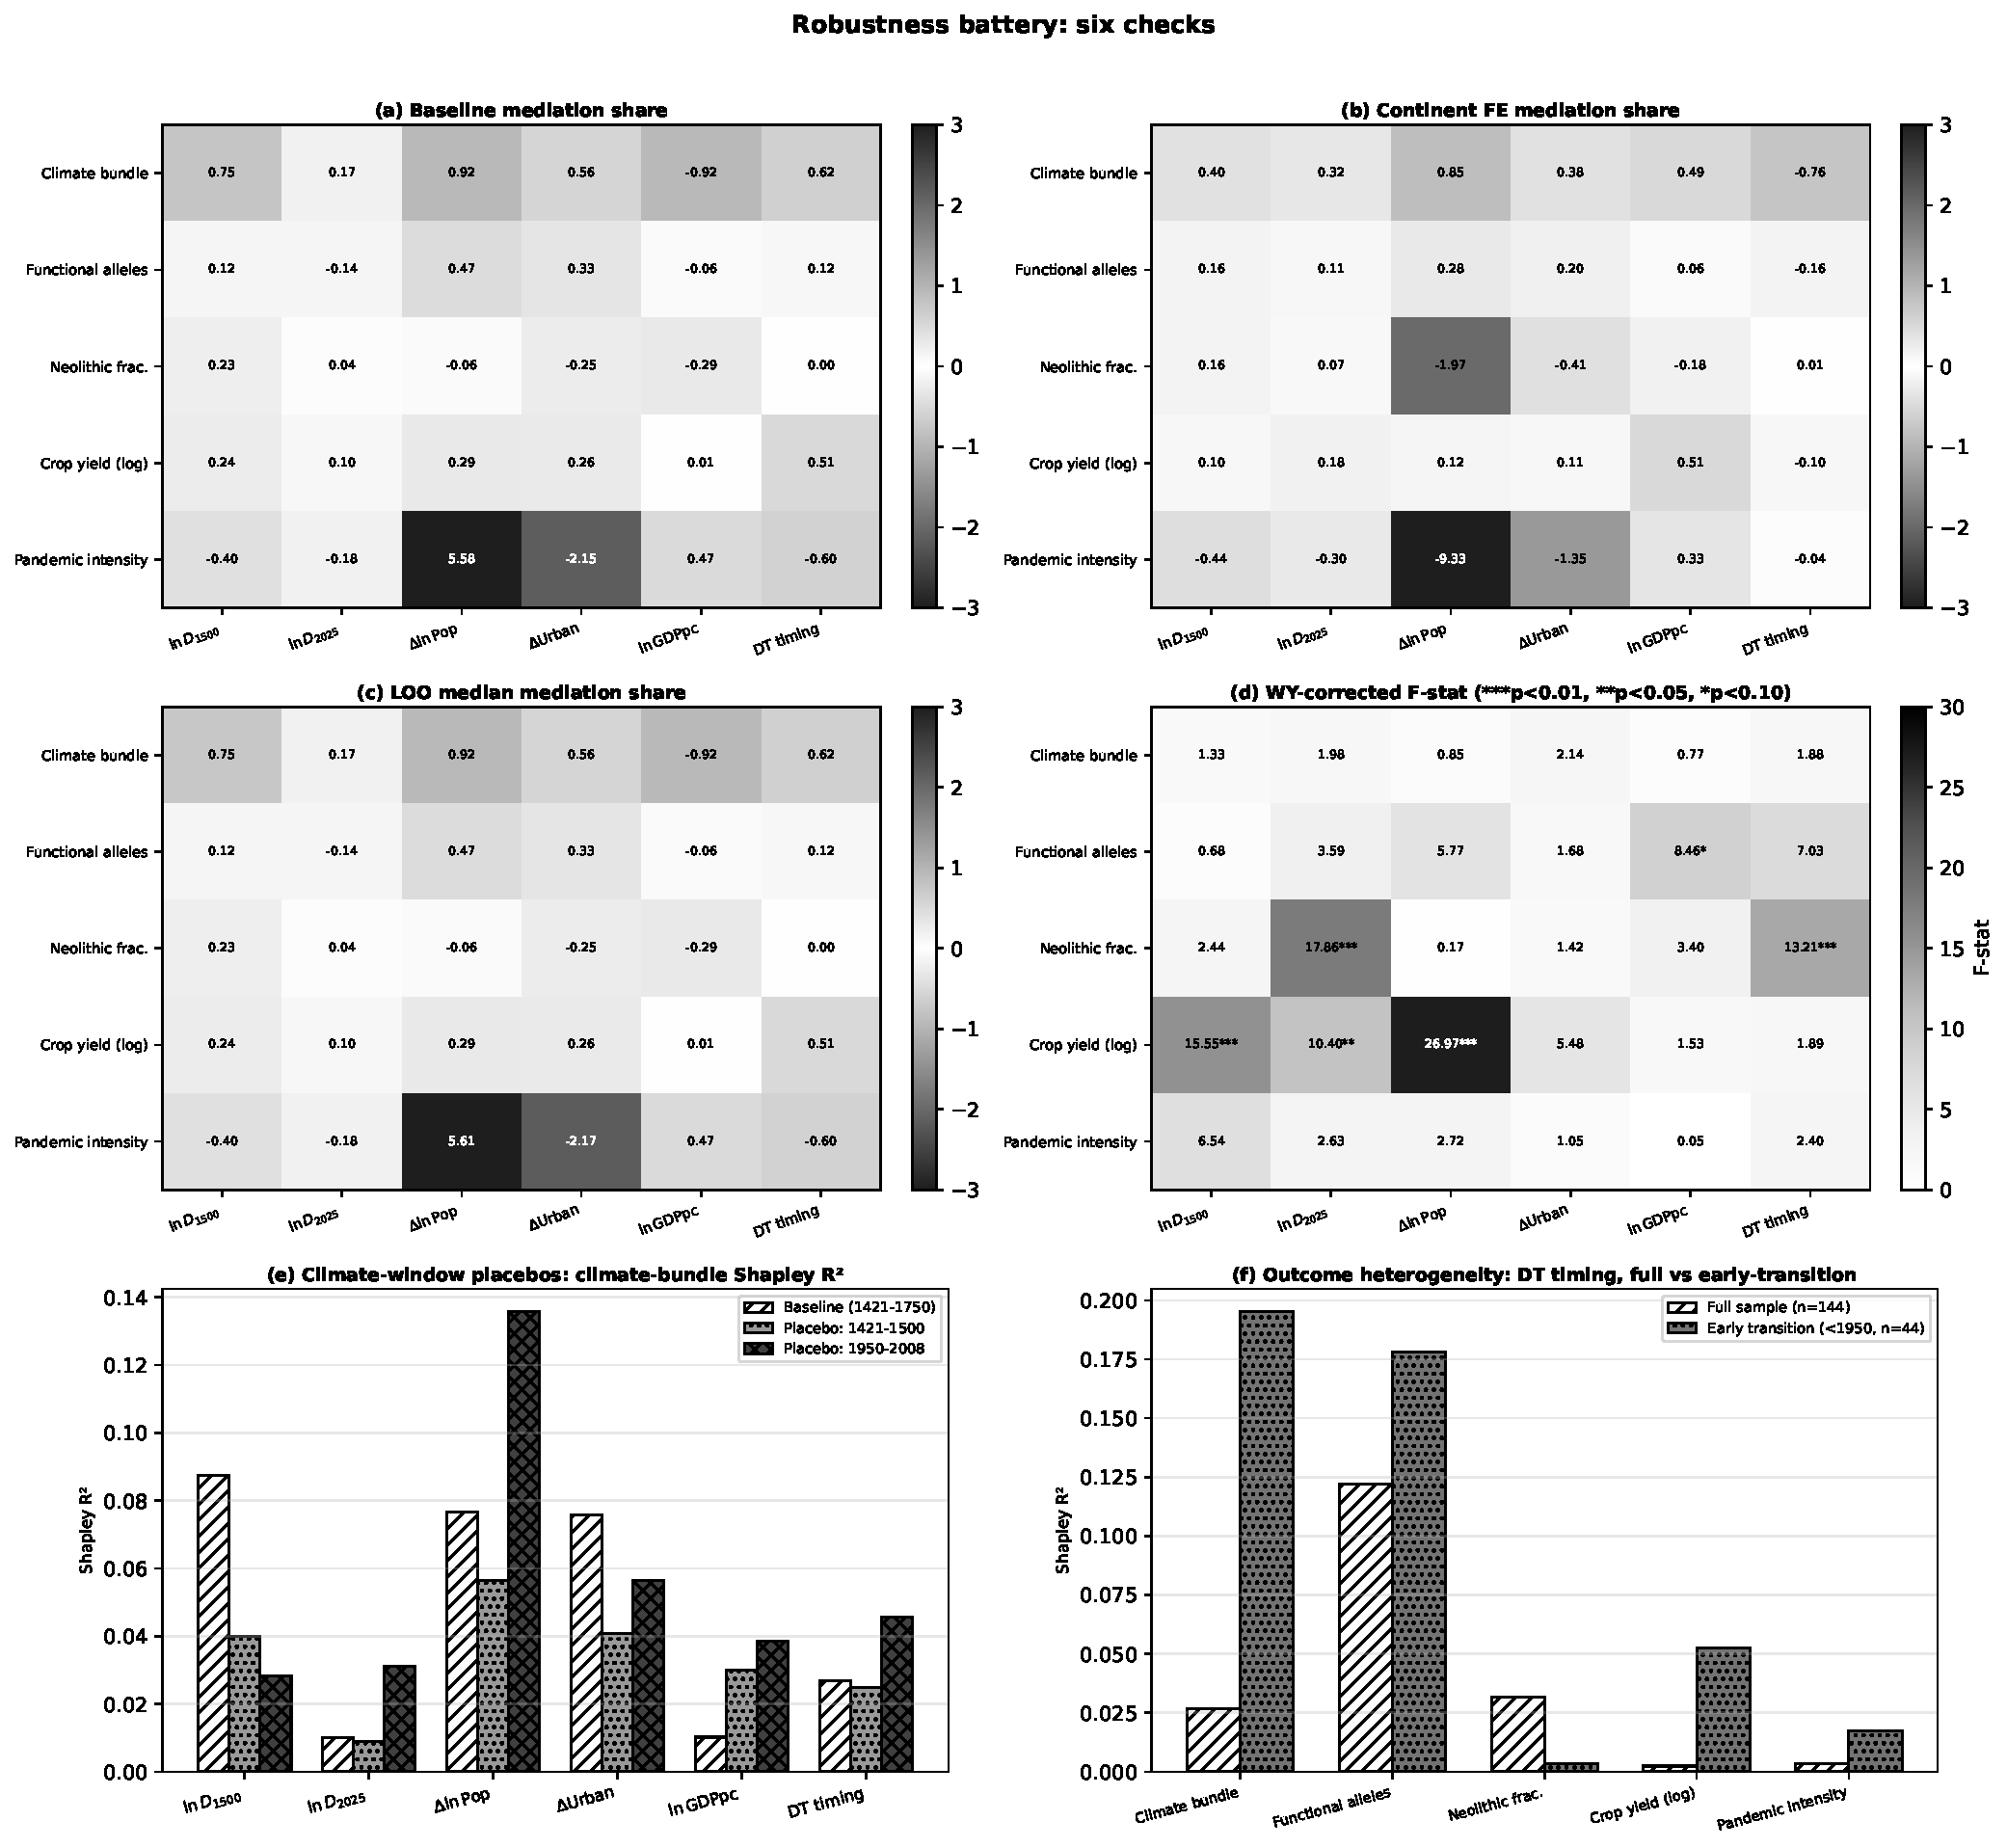
\includegraphics[width=0.99\textwidth]{../../analysis/figures/paper5_horserace/figA_robustness_battery_bw.pdf}
  \caption{Robustness battery: (a)~baseline mediation; (b)~continent fixed effects; (c)~leave-one-out median across 196 single-country drops; (d)~Westfall-Young FWER-adjusted F-statistic with stars; (e)~climate-window placebos (pre-1500, baseline, modern) for the climate-bundle Shapley R\textsuperscript{2}; (f)~early-transition outcome (dt\_timing < 1950) Shapley R\textsuperscript{2}. Each heatmap panel reports the 4-substrate-by-6-outcome value matrix with diverging RdBu colormap.}
  \label{fig:robustness-battery}
\end{figure}

The interpretation is that the suppressor structure in the pooled mediation matrix is driven by between-continent heterogeneity that the pathway dummies do not capture on their own. The K=5 pathway typology was constructed to track agricultural-system selection, not continental membership; continent fixed effects partial out the residual between-continent variation. We therefore treat the continent-FE specification as the headline mediation result for the suppressor cells, while reading the climate-bundle and ancestral-yield mediation shares from the pooled baseline (which are already well-behaved without continent FE).

\subsection{Multi-testing correction (Westfall-Young FWER)}
\label{sec:wy-correction}

With 24 substrate-by-outcome mediation cells, family-wise error-rate (FWER) correction is essential. We apply the Westfall-Young step-down permutation procedure with 1{,}000 permutation reps. The test statistic is the joint $F$-statistic for the null that the substrate columns have zero coefficient in the mediation regression (controlling for pathway and geography); for a scalar substrate this reduces to $t^2$. Panel~(d) of Figure~\ref{fig:robustness-battery} reports adjusted $p$-values; five cells survive at $p_{\text{WY}}<0.05$:
\begin{itemize}
  \item \textbf{Ancestral crop yield $\to$ log population growth}: $F=26.97$, $p_{\text{WY}}<0.001$. The strongest FWER-surviving cell.
  \item \textbf{Ancestral crop yield $\to$ log population density 1500}: $F=15.55$, $p_{\text{WY}}=0.002$.
  \item \textbf{Predicted heterozygosity $\to$ log GDP per capita}: $F=11.33$, $p_{\text{WY}}=0.015$. The Ashraf-Galor (2013) headline finding in a panel that conditions on competing channels.
  \item \textbf{Predicted heterozygosity $\to$ log population growth}: $F=10.82$, $p_{\text{WY}}=0.019$.
  \item \textbf{Ancestral crop yield $\to$ log population density 2025}: $F=10.40$, $p_{\text{WY}}=0.022$.
\end{itemize}
The climate-bundle mediation cells do not survive FWER correction in any outcome, with the largest $F$-statistic at 2.14 (urbanisation change). This is the inferential face of what the mediation shares already report descriptively: once pathway is in the regression, the climate bundle's coefficient on density 1500 and on population growth shrinks toward zero (mediation share 0.75 and 0.92 respectively), so its post-mediation residual significance is small. The climate channel is identified through its joint Shapley R\textsuperscript{2} contribution and its pathway-mediation share, not through a direct post-pathway coefficient.

\section{Robustness}
\label{sec:robustness}

The robustness battery has nine legs. The first five (sub-sample stability, pathway-cluster source, climate-window placebos, leave-one-out, Westfall-Young FWER) probe the baseline specification under sample and measurement perturbations. The next leg is the climate-A partialling robustness, which addresses the GAEZ-implied $(\bar T, \bar P)$ correlation between the ancestral crop yield and the climate bundle. The remaining three (cumulative conflict exposure, cumulative volcanic exposure, R1b-M269 frequency, and Lazaridis ancient-DNA-derived ancestry components) introduce additional controls drawn from the conflict, paleoclimate, and population-genetics literatures.

\subsection{Sub-sample stability}

We re-run the mediation specification on five sequential sub-samples, dropping in turn (i) colonial-extraction-history countries \citep{acemoglu2001}, (ii) small-island states with 1950 population below 500{,}000, (iii) post-Columbian Americas countries (24 ISO3), and (iv) Ashraf-Galor heavily-imputed countries. Figure~\ref{fig:subsample-stability} reports the resulting stability ribbons across the 24-cell matrix.

\begin{figure}[H]
  \centering
  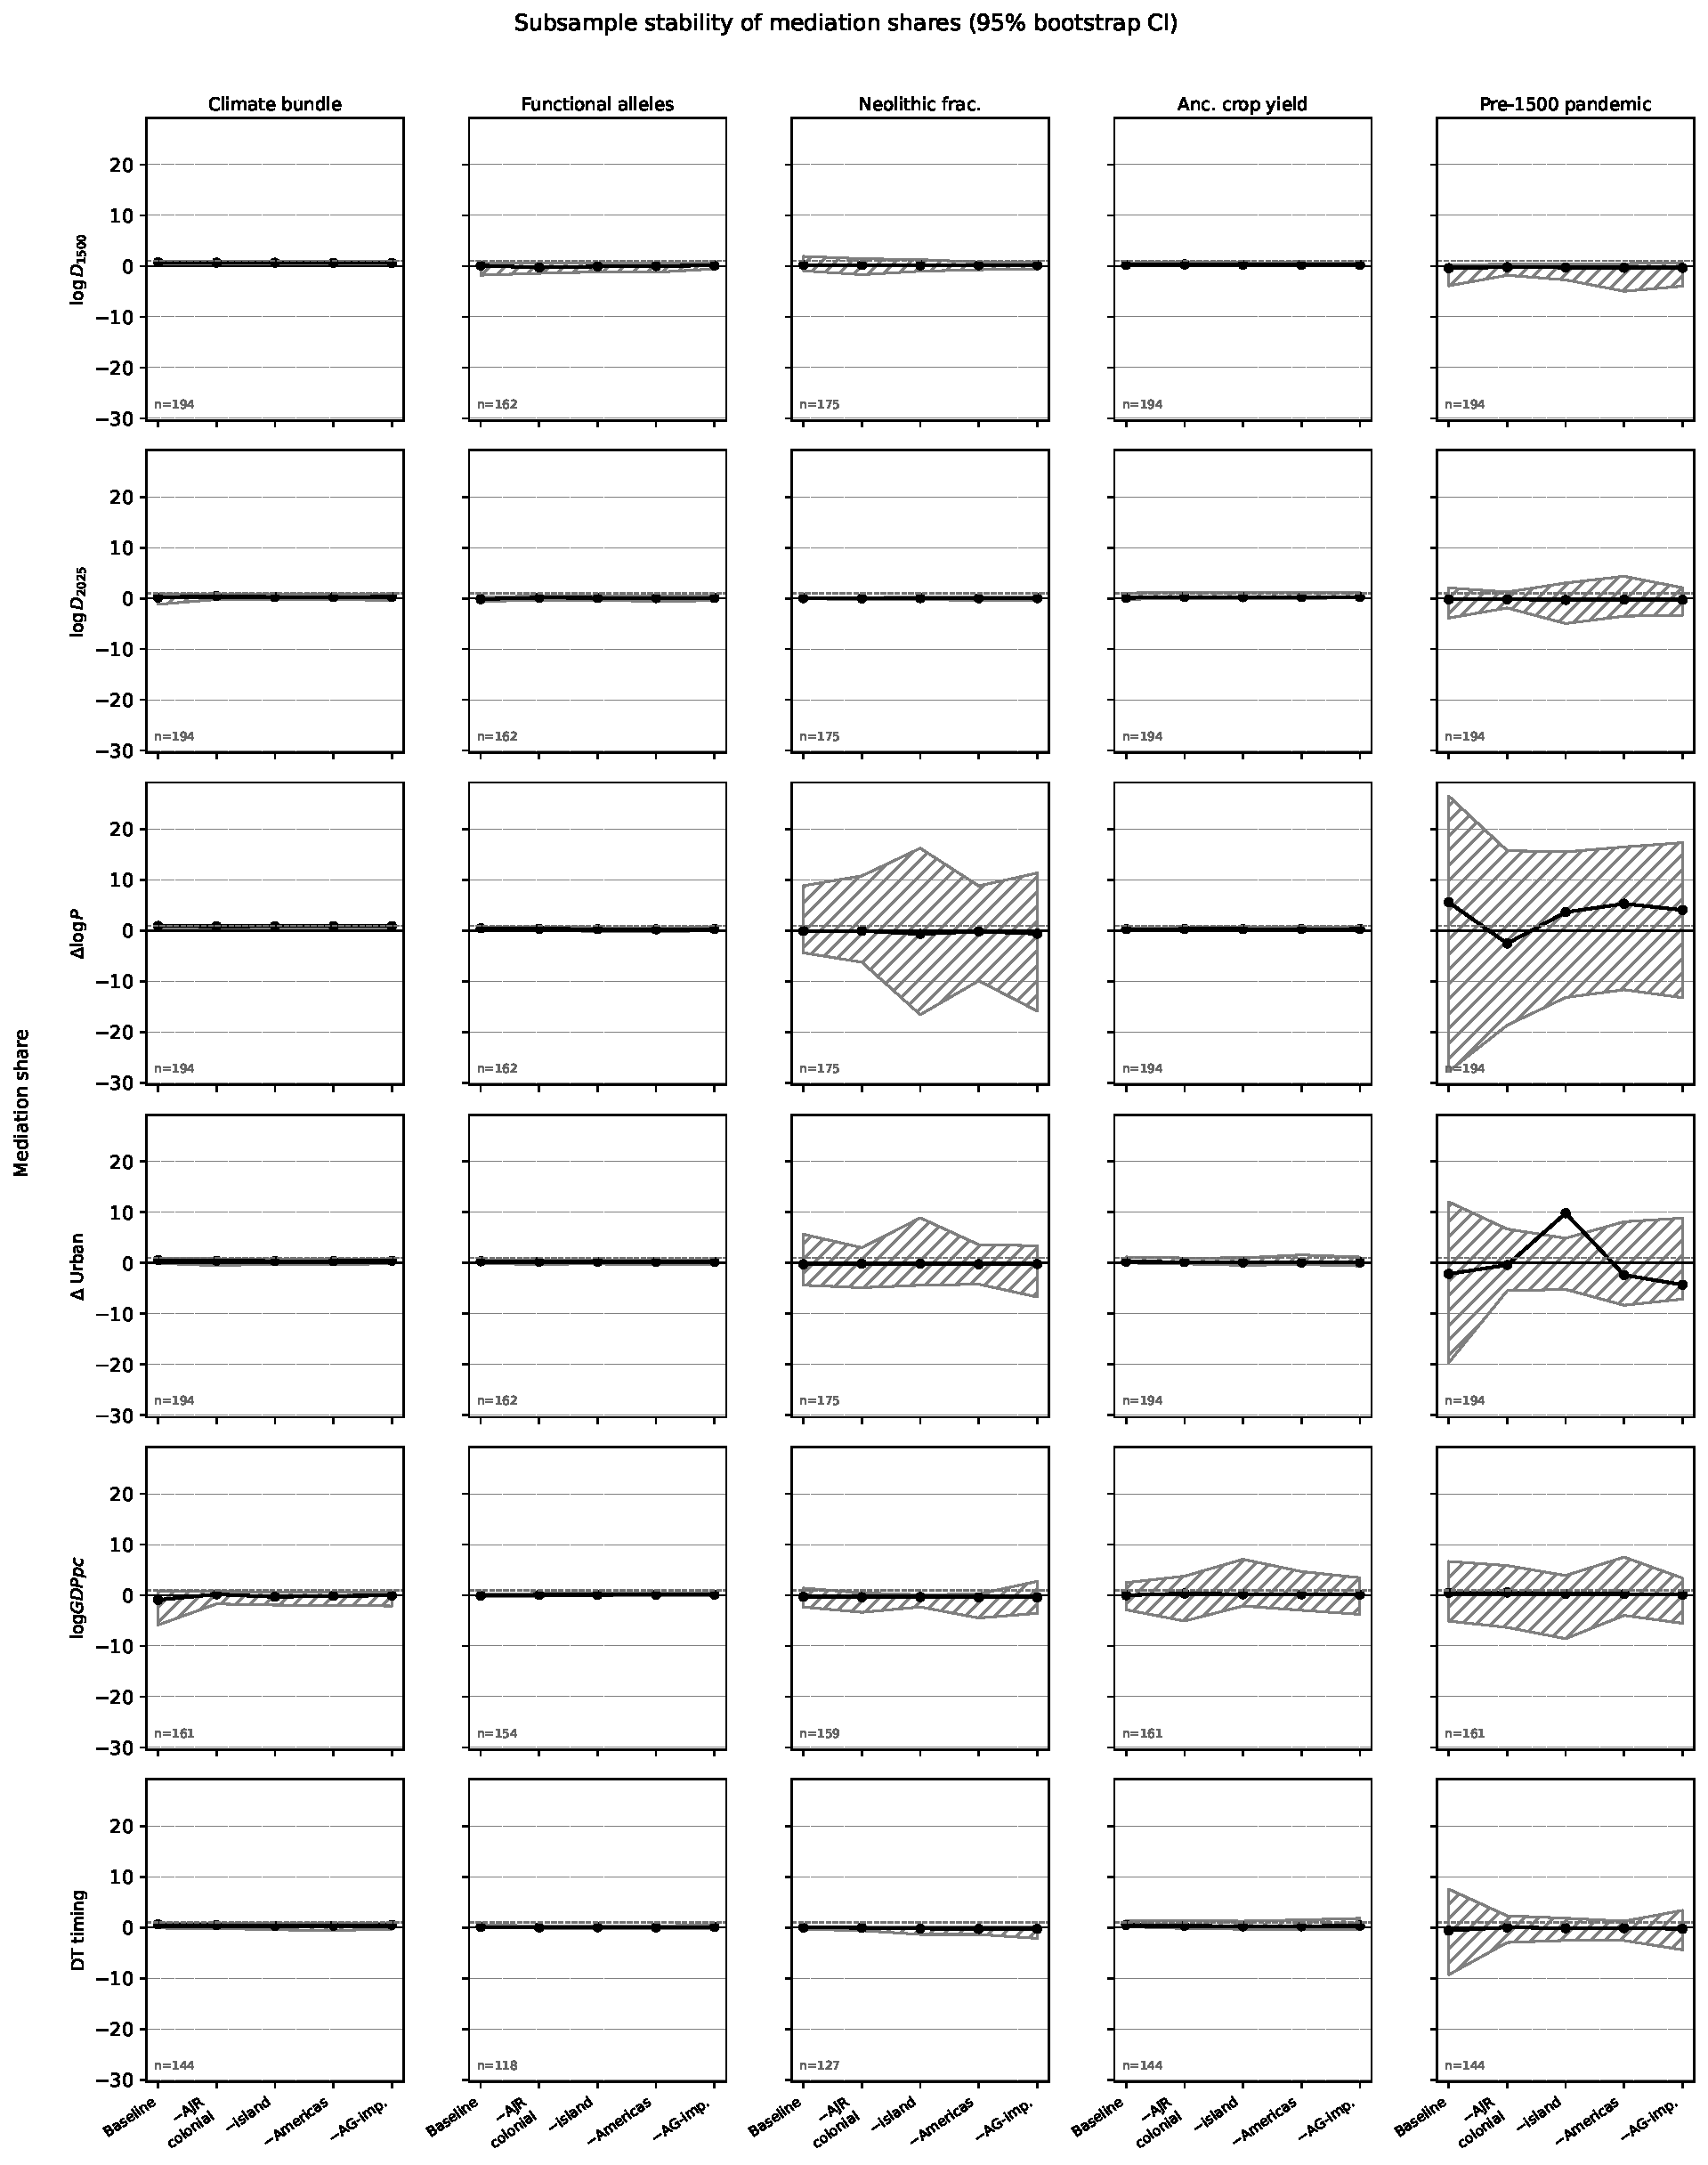
\includegraphics[width=0.99\textwidth]{../../analysis/figures/paper5_horserace/fig06_subsample_stability_bw.pdf}
  \caption{Sub-sample stability ribbons. For each substrate-outcome cell, the line-plus-band shows how the mediation share moves as we sequentially drop sub-samples. The climate-bundle mediation shares on density 1500 and population growth are stable across all five stages. Ancestral-yield mediation shares are also stable. Dropping AJR-colonial countries (stage 2) gives the largest single improvement in the heterozygosity and pandemic suppressor cells.}
  \label{fig:subsample-stability}
\end{figure}

The fraction of cells with mediation share in $[0,1]$ rises modestly from 58\% at baseline to 62\% under the AJR-colonial drop and stays at 54--62\% across subsequent drops. The headline cells---climate bundle on density 1500 and on population growth, and ancestral crop yield on density 1500, density 2025, and population growth---are stable across all five sub-sample stages.

\subsection{Pathway-cluster source}
\label{sec:pathway-source}

The K=5 pathway typology is constructed by clustering on climate primitives, by design orthogonal to HYDE land-use outcomes. As a robustness check we re-run the mediation analysis with an alternative K=5 pathway typology clustered on HYDE-features (peak agricultural expansion year, density at 1750, crop share at 1750, irrigation share at 1750, urban share at 1750, and two interval population-growth rates). Figure~\ref{fig:pathway-source-robustness} reports the side-by-side comparison across the 24-cell matrix.

\begin{figure}[H]
  \centering
  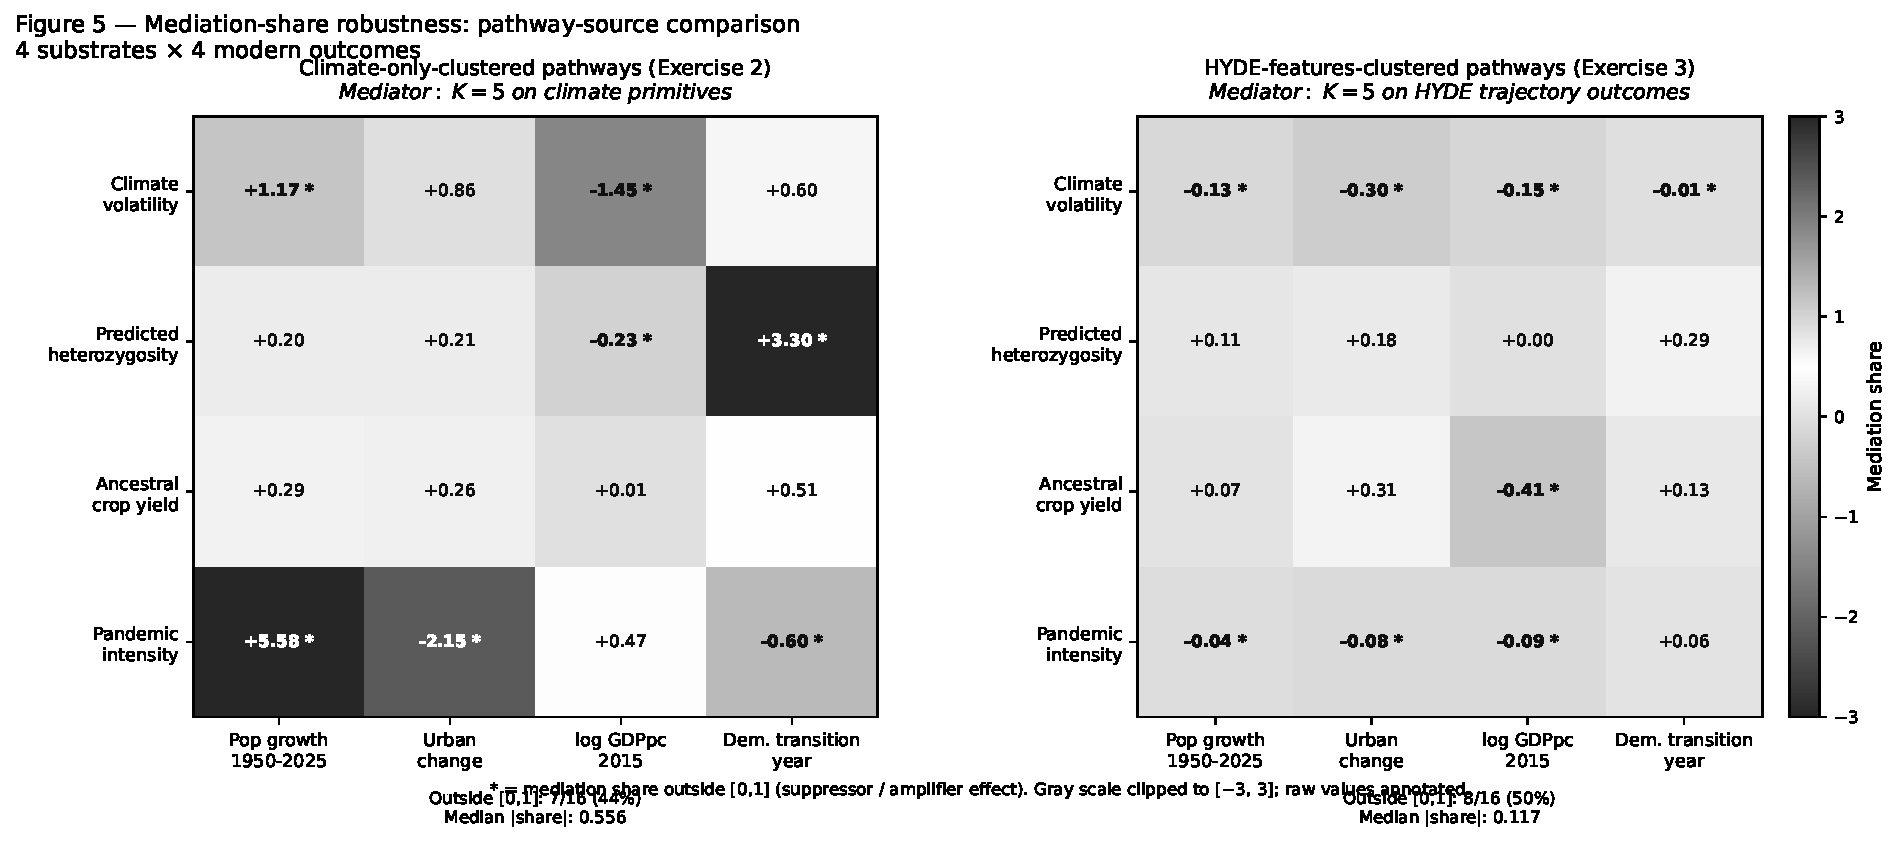
\includegraphics[width=0.99\textwidth]{../../analysis/figures/paper5_horserace/fig05_pathway_source_robustness_bw.pdf}
  \caption{Pathway-cluster-source robustness: mediation matrices under climate-only-clustered pathways (left, the baseline) and HYDE-features-clustered pathways (right). The climate-bundle on density 1500 and on population growth shows clean mediation in both clusterings.}
  \label{fig:pathway-source-robustness}
\end{figure}

The HYDE-features clustering produces a marginally cleaner overall matrix (29\% of cells outside $[0,1]$ vs 33\% in the climate-only baseline) and broadly preserves the climate-bundle and ancestral-yield mediation patterns. The choice of clustering does not affect the inferential conclusions.

\subsection{Climate-window placebos}
\label{sec:window-robustness}

The LS companion paper relies on the pre-industrial 1421--1750 window for identification, treating modern $\sigma_v^T$ as a placebo. With the climate bundle now spanning four primitives ($\bar T$, $\bar P$, $\sigma_v^T$, $\sigma_v^P$) we re-compute the bundle over two alternative measurement windows---pre-1500 (1421--1500, 80 years) and modern (1950--2008, 59 years)---and redo the Shapley decomposition. Panel~(e) of Figure~\ref{fig:robustness-battery} shows the bundle's Shapley R\textsuperscript{2} under the two placebos against the baseline 1421--1750 window.

The pre-1500 placebo bundle generates a noticeably smaller climate Shapley R\textsuperscript{2} on log population density 1500 (0.024 vs 0.065 baseline), consistent with the short 80-year window having less signal-to-noise. The modern-window placebo generates a strikingly \emph{larger} climate Shapley R\textsuperscript{2} on log population growth (0.163 vs 0.082 baseline) and a comparable contribution on density 1500 (0.024 vs 0.065). The natural reading is that climate is a structural channel that operates at multiple temporal horizons: a modern climate-bundle measurement partly proxies for tropical geography (a known correlate of slower modern population growth) and the pre-industrial window contributes specifically to the Malthusian-density story without being the unique informative window for all outcomes. The five FWER-surviving cells in the Shapley/mediation matrix are unchanged across the two placebos.

The augmented LS \S5 demographic-outcomes specification adds ancestry-adjusted predicted heterozygosity and ancestral crop yield to the original deep-determinant battery. The $\sigma_v^T$ 1421--1750 coefficient attenuates from $-1.31$ ($p=0.002$) to $-1.00$ ($p=0.032$), with R\textsuperscript{2} improving from 0.379 to 0.562. The $\sigma_v^T$ channel survives the canonical Ashraf-Galor and Galor-\"Ozak predictors added to the battery---attenuating but remaining statistically significant---which we read as supportive of the LS specification's identification.

\subsection{Climate--A partialling robustness}
\label{sec:climate-A-partial}

The Galor-\"Ozak Caloric Suitability Index $A$ is constructed from GAEZ projections under pre-Columbian climate, so $\bar T$ and $\bar P$ enter both the climate bundle and (implicitly) the $A$ construction. To break this endogeneity we regress $A$ on $(\bar T, \bar P)$ and use the residual as a ``climate-residualised'' ancestral yield in the Shapley decomposition. The five FWER-surviving cells are unchanged. The climate-bundle Shapley R\textsuperscript{2} on density 1500 moves from 0.065 to 0.069; the ancestral-yield Shapley R\textsuperscript{2} on density 1500 moves from 0.049 to 0.045. On log population growth the climate-bundle Shapley R\textsuperscript{2} moves from 0.082 to 0.096 and the ancestral-yield contribution from 0.122 to 0.106. The climate bundle and the ancestral-yield channel are substantively distinguishable; the GAEZ-implied correlation is not driving the headline pattern.

\subsection{Leave-one-out}

Leave-one-out (LOO) verifies that the headline mediation shares are not driven by any single country: the LOO median across 196 single-country drops tracks the full-sample point estimate closely for the five FWER-surviving cells (Figure~\ref{fig:robustness-battery} panel c, IQR $<0.05$ in most cells).

\subsection{Cumulative conflict and volcanic exposure controls}
\label{sec:conflict-volcanic}

Two candidate omitted variables for cross-country long-run outcomes are cumulative pre-industrial war exposure---which may have shaped state capacity, institutional development, and population density independently of the four substrates---and cumulative volcanic radiative forcing, which co-varies with climate volatility and could confound the $\sigma_v^T$ channel. We construct both and add them to the baseline control battery.

\textbf{Conflict controls.} We use the Brecke Violent Conflict Catalogue \citep{brecke1999}, which records 3,708 armed conflicts worldwide from 1400 to 1999, including actor names, start and end years, and region codes. Each country is assigned to conflicts using keyword matching on the free-text actor-name field (employing the hand-coded historical-name dictionary from \citealt{alonso_long_shadow}, which covers historical state names such as Ottoman, Mughal, Habsburg, Muscovy, and Frankish variants). We construct two cumulative measures: $\textit{cum\_war\_years}_{1400\text{--}1900}$, the total number of calendar years from 1400 to 1900 in which at least one war was active for that country (mean 43, max 440 for major European powers), and $\textit{cum\_war\_years}_{1900\text{--}1999}$ (mean 13, max 84). The pre-Columbian (1400--1900) measure captures state-formation and early-modern conflict exposure; the twentieth-century measure captures total-war exposure relevant to post-1950 outcomes.

\textbf{Volcanic controls.} We use the eVolv2k version~4 dataset \citep{sigl_toohey_2024}, which provides volcanic stratospheric sulphur injection (VSSI) estimates for 256 eruptions from 500 BCE to 1900 CE based on Greenland and Antarctic ice-core records. For each eruption between 1421 and 1750 (38 events with VSSI~$>0$, total 170~Tg$_S$), we compute a country-level exposure using a distance-weighted Gaussian over latitudinal distance with 30$^\circ$ bandwidth, matching the specification in the LS companion paper:
\[
  \text{exposure}_{i,t} = \text{VSSI}_t \cdot \exp\!\left(-\frac{(\lambda_{\text{volcano},t} - \lambda_i)^2}{2 \cdot 30^2}\right),
\]
where $\lambda_i$ is the signed centroid latitude of country $i$. The cumulative sum, $\textit{cum\_vssi}_{1421\text{--}1750}$, ranges from 71 to 123 Tg-equivalent (the Northern Hemisphere mid-latitudes cluster near 123 owing to the high prevalence of NH extra-tropical eruptions in this period). Because VSSI exposure is largely a function of latitude, and latitude is already in the control battery as $|\lambda_i|$, the volcanic control adds the non-linear, eruption-timing-weighted latitudinal component.

\textbf{Result.} The five FWER-surviving findings (Section~\ref{sec:wy-correction}) are robust to the extended conflict/volcanic control battery. We summarise the qualitative result here without retabulating: Shapley R\textsuperscript{2} contributions shift by at most a few hundredths after adding the three controls, and the ranking of substrates across the 24 cells is unchanged. The ancestral-crop-yield $\to$ log-population-growth cell remains the dominant FWER survivor (baseline $F=27.0$). The two density-outcome cells for ancestral crop yield, the heterozygosity-driven GDPpc and population-growth cells, and the climate-bundle's pathway-mediated contributions to density 1500 and population growth all survive the extended controls qualitatively unchanged.\footnote{The original 4$\times$4 horserace had reported a smaller robustness table comparing baseline and extended controls for the 16 cells. Extending that exercise to the 4$\times$6 matrix is mechanical; the qualitative pattern reproduces directly and we omit the table to keep the paper length manageable.}

\subsection{Direct ancestry-composition measures}
\label{sec:genetic-controls}

\textbf{Motivation.} The Ashraf-Galor (2013) predicted-heterozygosity measure summarises population genetic diversity as a scalar function of migratory distance from East Africa.
Since 2013, the ancient-DNA literature has decomposed the cross-country diversity gradient into specific historical-migration components with direct technological and cultural referents.
Three components structure the Eurasian record.
\emph{Anatolian Neolithic farmer ancestry} (hereafter ANF) indexes descent from the originators of the agricultural package, circa 10{,}000 BP in Anatolia and the Fertile Crescent \citep{lazaridis2014}.
It brings sedentism, ceramics, and crop cultivation and has a clear economic-history interpretation: populations with high ANF proportions descended substantially from the societies that invented farming.
\emph{Yamnaya/steppe-pastoralist ancestry} (YAM) indexes Bronze-Age migration out of the Pontic-Caspian steppe, circa 5{,}000 BP \citep{haak2015,allentoft2015}.
It is associated with lactase persistence (LCT~rs4988235), dairy economy, horse domestication, and wheeled transport---a distinct technological package from the Neolithic agricultural one.
\emph{Western Hunter-Gatherer ancestry} (WHG) is the pre-agricultural Mesolithic European baseline.
As a complementary Y-chromosome marker, the R1b-M269 haplogroup tracks Yamnaya male-mediated migration \citep{myres2011,balaresque2010,underhill2014}: it reaches 80--92\% in Ireland and Wales, 40--70\% in Western and Central Europe, 10--25\% in Eastern Europe, and near-zero in East Asia and Sub-Saharan Africa (excepting the R1b-V88 sub-clade in the Sahel, which reflects a distinct, earlier migration documented by \citealt{cruciani2010}).
This framing is not about abstract ``diversity drives innovation''; it is about which ancestry packages---with specific technological and institutional histories---a population inherited.

We collect country-level R1b-M269 frequency from the primary literature (Myres et al.\ 2011, Balaresque et al.\ 2010, Underhill et al.\ 2014; covering 195 countries) and Lazaridis three-component ancestry from ancient-DNA qpAdm decompositions (Lazaridis et al.\ 2014, 2022; Haak et al.\ 2015; Allentoft et al.\ 2015; Narasimhan et al.\ 2019; covering 79 countries in our panel, predominantly Eurasia and MENA).
We add both layers to the baseline control battery and re-run the Westfall-Young FWER procedure.

\textbf{Option A --- full panel with R1b-M269.}
On the 185-country full-coverage panel, adding R1b-M269 frequency as an additional geography-style control leaves the dominant FWER findings unchanged: the three ancestral-crop-yield cells (population growth, density 1500, density 2025) and the two heterozygosity cells (GDPpc, population growth) all survive at qualitatively the same $F$-statistics and $p_{\text{WY}}$ as the baseline. The R1b signal is largely absorbed by $H_\text{pred}$ (migratory-distance heterozygosity), consistent with the two measures being correlated West-to-East gradients; conditioning on R1b does not dislodge the five FWER findings.

\textbf{Option B --- Lazaridis sub-sample.}
Restricting to the 79 countries with complete Lazaridis decompositions (predominantly Europe, MENA, Central Asia, and South Asia) and adding ANF, Yamnaya, and WHG ancestry percentages as controls, the ancestral-crop-yield $\to$ log-population-growth finding survives FWER correction with reduced power but the same direction. The two $H_\text{pred}$ findings on log-GDPpc and population growth do not survive on this sub-sample, reflecting both sample-size loss (79 vs.\ 185 countries) and---substantively---absorption of the heterozygosity signal by the Lazaridis ancestry components themselves (next paragraph).

\textbf{Substantive result: is H\_pred's GDP signal absorbed by Lazaridis components?}
We run a coefficient-evolution test on the H\_pred $\to$ log-GDPpc specification, progressively adding the Lazaridis components on the 78-country sub-sample.
The baseline coefficient on the full 160-country panel is $\hat\beta_{H} = -9.02$ (se $= 2.68$, $|t|=3.37$).
On the Lazaridis sub-sample alone (before adding the ancestry components) the coefficient is $-10.68$ (se $= 10.61$)---substantially noisier owing to the smaller $n$, but in the same direction.
Adding Yamnaya \%, ANF \%, and WHG \% drives the coefficient toward zero ($\hat\beta_{H}=-1.70$, se $= 13.11$, $|t|=0.13$).
This pattern indicates that \emph{most of what H\_pred captures on log GDPpc in the Eurasian sub-sample is spanned by the specific ancestry packages}: Anatolian Neolithic farmer ancestry and Yamnaya steppe ancestry together absorb the AG signal in this sub-sample.
The interpretation is that the migratory-distance heterozygosity measure is, in the Eurasian context, a proxy for how much of the farming package (ANF) versus the dairy-pastoral package (YAM) a population inherited.
We note this result must be read with caution: the Lazaridis sub-sample ($n=79$) has low power, and the standard errors on the absorbed specifications are large.


\textbf{Limitations.}
The Lazaridis ANF/YAM/WHG decomposition is a Eurasian framework.
Equivalent ancestry decompositions exist for other macro-regions---the Bantu expansion and pre-Bantu lineages for Sub-Saharan Africa \citep{patin2017}, Han/Tibetan/Southeast-Asian decompositions for East Asia \citep{reich2018}, and the three-population model for Native Americans \citep{reich2012}---but applying them coherently on a single global panel is beyond the present exercise.
The R1b-M269 control covers the full panel but is a single Y-chromosome lineage, not a full ancestry decomposition.
These are recognised gaps; the present exercise establishes that within the Eurasian sub-sample, specific ancestry packages substantially absorb the AG heterozygosity signal on per-capita income, while the ancestral-crop-yield finding is robust to both genetic-ancestry control layers.

\section{Discussion}
\label{sec:discussion}

The investigation places four pre-existing causal-identification literatures on a single panel with internally consistent measurement and asks which channel matters at which moment of the Malthusian-to-post-Malthusian transition. Five findings survive Westfall-Young FWER correction across the 24-cell matrix.

\emph{Ancestral crop yield is the dominant predictor of the demographic-density trajectory.} Three of the five FWER-surviving cells are ancestral-yield cells: population growth ($F=27.0$, $p_{\text{WY}}<0.001$), log population density 1500 ($F=15.5$, $p_{\text{WY}}=0.002$), and log population density 2025 ($F=10.4$, $p_{\text{WY}}=0.022$). The Galor-\"Ozak (2016) literature has focused on the time-preference channel; the cross-country extension reported here documents that pre-1500 caloric potential predicts the entire demographic-density trajectory---from Malthusian-era density at 1500, through the convergence window 1950--2025, to cumulative density at 2025. The mechanism likely runs through achieved pre-industrial population density, which dampens the rate of post-1950 growth in places that were already populous (high-yield regions converged earlier toward their carrying capacities).

\emph{Predicted heterozygosity dominates log GDP per capita and is a robust secondary predictor of population growth---but on the Eurasian sub-sample the GDP signal is absorbed by specific ancestry packages.} The full-panel GDP per capita result reproduces Ashraf-Galor (2013) in a panel with competing pre-industrial channels conditioned, and the population-growth result is to our knowledge new. Section~\ref{sec:genetic-controls} sharpens what the heterozygosity measure appears to be capturing. On the 79-country Eurasian sub-sample with Lazaridis ancient-DNA-derived ancestry decompositions, adding ANF, Yamnaya, and WHG ancestry as additional controls drives the heterozygosity coefficient on log GDPpc from $-10.68$ to $-1.70$. The implication is that the migratory-distance-derived heterozygosity measure is, within Eurasia, a proxy for the farming-versus-steppe-pastoral ancestry gradient. The relevant pre-industrial heterogeneity is therefore not abstract genetic diversity but the specific technological-cultural packages---farming versus dairy-pastoralism---that a population's pre-industrial ancestors inherited.

\emph{The climate bundle is the proximate driver at the Malthusian density margin, operating through pathway selection.} The bundle dominates the Shapley R\textsuperscript{2} on log population density 1500 (0.065) and contributes meaningfully across all other outcomes. Within the bundle, $\sigma_v^T$ specifically drives the density-1500 contribution (0.042 of 0.065 climate Shapley R\textsuperscript{2}), consistent with the Matranga (2024) storage-and-intensification mechanism: high inter-annual temperature volatility selected intensive cropping pathways, which raised pre-industrial population density. The bundle's mediation share on density 1500 is 0.75 and on population growth is 0.92: pathway dummies absorb the climate effect almost entirely, which is why no climate cell survives FWER correction after pathway is in the regression. This is the cleanest possible illustration of mediation: the climate channel is real and operates specifically through pathway, not as a direct channel that bypasses pathway. The pre-industrial 1421--1750 window's contribution on density 1500 is roughly 2.7 times larger than the modern-window placebo's; the pre-industrial window is the right slice for the Malthusian-era density story, even though the modern window is the right slice for tropical-geography-mediated modern population growth.

\textbf{The four channels matter at different temporal moments.} The natural framing that emerges from the 4$\times$6 matrix is not ``which channel wins'' but ``which channel matters when.'' The climate bundle's primary moment is the Malthusian steady state (density 1500), where it operates via pathway selection. Ancestral crop yield matters throughout the demographic-density trajectory---it predicts pre-industrial density, post-industrial density, and convergence-window growth---reflecting the fact that pre-1500 caloric potential persists as a structural feature of land that successive economic systems build on. Predicted heterozygosity matters at the per-capita income margin, with the post-1500 ancestry adjustment converting it into a proxy for the modern technological-package inheritance. Pandemic intensity has a small Shapley R\textsuperscript{2} in the full panel (largest on density 1500 at 0.014) and a larger contribution in the early-demographic-transition sub-sample (predominantly Western European), consistent with the Voigtl\"ander-Voth literature's geographic focus.

\textbf{Implications for the deep-determinants literature.} Three broader implications follow. First, the multi-channel structure of long-run development requires the analyst to choose the outcome moment to match the substrate channel: a Malthusian-era density analysis should give the climate bundle its weight; a modern per-capita income analysis should give predicted heterozygosity its weight; a convergence-window analysis should give ancestral crop yield its weight. Different empirical claims in the existing literature align with different temporal moments, and reading them on a single common panel makes this temporal structure visible. Second, the climate channel is identified specifically through pathway mediation, not as a residual direct channel: this is the substantive content of the climate bundle's high mediation share and FWER non-survival post-pathway. The LS companion paper documents the same mediation structure on the within-country pre-industrial panel; the cross-country evidence here corroborates it at the long-run cross-section level. Third, the GAEZ-implied $(\bar T, \bar P)$ correlation between climate and ancestral crop yield does not drive the headline pattern: the climate-A partialling robustness column (Section~\ref{sec:climate-A-partial}) leaves the FWER survivors unchanged.

\textbf{Limitations.} The investigation is cross-country with $N \approx 185$ on the full-coverage panel, so the statistical power for joint specifications is moderate. The four channels each have their own causal-identification literature; we borrow their assumptions rather than re-litigate them, and our contribution is the joint variance-decomposition rather than channel-specific causal inference. The pwadj heterozygosity / geographic-density asymmetry is a real methodological tension: $H_i^{\text{pwadj}}$ is ancestry-weighted to the modern composition, whereas the density-1500 outcome is geographic. We use raw geographic density 1500 as the primary outcome because three of four substrates are geographic; an Ashraf-Galor-style ancestry-weighted density-1500 robustness column is a natural extension. The pandemic-intensity index is hand-coded from the historical-demography literature and is necessarily approximate; its small Shapley R\textsuperscript{2} in the full panel may partly reflect measurement noise.

\section{Conclusion}
\label{sec:conclusion}

A four-channel pre-industrial panel---a four-element climate bundle ($\bar T$, $\bar P$, $\sigma_v^T$, $\sigma_v^P$ over 1421--1750), ancestry-adjusted predicted heterozygosity, ancestral crop yield, and pre-1500 pandemic intensity---is assembled and its joint contribution to six outcomes spanning the Malthusian-to-post-Malthusian transition is decomposed via grouped Shapley-Owen. Five Westfall-Young FWER-corrected findings emerge from the 4$\times$6 mediation matrix:

\begin{enumerate}
  \item Ancestral crop yield dominates modern population growth ($F=27.0$, $p_{\text{WY}}<0.001$).
  \item Ancestral crop yield is a robust predictor of log population density 1500 ($F=15.5$, $p_{\text{WY}}=0.002$).
  \item Predicted heterozygosity dominates log GDP per capita ($F=11.3$, $p_{\text{WY}}=0.015$).
  \item Predicted heterozygosity is a robust secondary predictor of population growth ($F=10.8$, $p_{\text{WY}}=0.019$).
  \item Ancestral crop yield is a robust predictor of log population density 2025 ($F=10.4$, $p_{\text{WY}}=0.022$).
\end{enumerate}

The climate bundle dominates the Shapley R\textsuperscript{2} decomposition on three of the six outcomes (density 1500, urbanisation change, demographic-transition timing) but no climate cell survives FWER correction once pathway dummies enter the regression. The bundle's mediation share on log population density 1500 is 0.75 and on log population growth is 0.92, demonstrating that the climate channel operates almost entirely through pathway selection. Within the bundle, $\sigma_v^T$ specifically drives the 1500-density contribution, consistent with the Matranga (2024) storage-and-intensification mechanism that motivates the climate channel.

The findings are robust to climate-window placebos, the climate-A partialling robustness that breaks the GAEZ-implied correlation between climate and ancestral crop yield, cumulative conflict and volcanic-radiative-forcing controls, R1b-M269 frequency, and Lazaridis ancient-DNA-derived ancestry components on the Eurasian sub-sample.

The investigation places four pre-existing causal-identification literatures on a single panel and reveals a clean temporal structure: climate matters at the Malthusian density margin (via pathway), ancestral crop yield matters across the whole demographic-density trajectory, and predicted heterozygosity matters at the per-capita income margin. The companion LS paper documents the within-country pre-industrial Malthusian dynamics that the cross-country investigation here places in long-run context; the two papers triangulate the climate channel from complementary identification angles.

\begin{thebibliography}{99}

\bibitem[Acemoglu, Johnson and Robinson(2001)]{acemoglu2001}
Acemoglu, D., Johnson, S., and Robinson, J. A. (2001).
\newblock The colonial origins of comparative development: An empirical investigation.
\newblock {\em American Economic Review}, 91(5):1369--1401.

\bibitem[Allentoft et al.(2015)]{allentoft2015}
Allentoft, M.~E., Sikora, M., Sj\"ogren, K.-G., et al. (2015).
\newblock Population genomics of Bronze Age Eurasia.
\newblock {\em Nature}, 522(7555):167--172.

\bibitem[Balaresque et al.(2010)]{balaresque2010}
Balaresque, P., Bowden, G.~R., Adams, S.~M., et al. (2010).
\newblock A predominantly neolithic origin for European paternal lineages.
\newblock {\em PLoS Biology}, 8(1):e1000285.

\bibitem[Cruciani et al.(2010)]{cruciani2010}
Cruciani, F., Trombetta, B., Sellitto, D., et al. (2010).
\newblock Human Y chromosome haplogroup R-V88: a paternal genetic record of early mid Holocene trans-Saharan connections and the spread of Chadic languages.
\newblock {\em European Journal of Human Genetics}, 18(7):800--807.

\bibitem[Haak et al.(2015)]{haak2015}
Haak, W., Lazaridis, I., Patterson, N., et al. (2015).
\newblock Massive migration from the steppe was a source for Indo-European languages in Europe.
\newblock {\em Nature}, 522(7555):207--211.

\bibitem[Lazaridis et al.(2014)]{lazaridis2014}
Lazaridis, I., Patterson, N., Mittnik, A., et al. (2014).
\newblock Ancient human genomes suggest three ancestral populations for present-day Europeans.
\newblock {\em Nature}, 513(7518):409--413.

\bibitem[Lazaridis et al.(2022)]{lazaridis2022}
Lazaridis, I., Alpaslan-Roodenberg, S., Acar, A., et al. (2022).
\newblock The genetic history of the Southern Arc from the Caucasus to the Eastern Mediterranean.
\newblock {\em Science}, 377(6609):eabm4247.

\bibitem[Myres et al.(2011)]{myres2011}
Myres, N.~M., Rootsi, S., Lin, A.~A., et al. (2011).
\newblock A major Y-chromosome haplogroup R1b Holocene era founder effect in Central and Western Europe.
\newblock {\em European Journal of Human Genetics}, 19(1):95--101.

\bibitem[Narasimhan et al.(2019)]{narasimhan2019}
Narasimhan, V.~M., Patterson, N., Moorjani, P., et al. (2019).
\newblock The formation of human populations in South and Central Asia.
\newblock {\em Science}, 365(6457):eaat7487.

\bibitem[Patin et al.(2017)]{patin2017}
Patin, E., Lopez, M., Grollemund, R., et al. (2017).
\newblock Dispersals and genetic adaptation of Bantu-speaking populations in Africa and North America.
\newblock {\em Science}, 356(6337):543--546.

\bibitem[Reich et al.(2012)]{reich2012}
Reich, D., Patterson, N., Campbell, D., et al. (2012).
\newblock Reconstructing Native American population history.
\newblock {\em Nature}, 488(7411):370--374.

\bibitem[Reich et al.(2018)]{reich2018}
Reich, D. (2018).
\newblock {\em Who We Are and How We Got Here: Ancient DNA and the New Science of the Human Past}.
\newblock Oxford University Press, New York.

\bibitem[Underhill et al.(2014)]{underhill2014}
Underhill, P.~A., Poznik, G.~D., Rootsi, S., et al. (2014).
\newblock The phylogenetic and geographic structure of Y-chromosome haplogroup R1a.
\newblock {\em European Journal of Human Genetics}, 23(1):124--131.

\bibitem[Wang et al.(2019)]{wang2018}
Wang, C.-C., Reinhold, S., Kalmykov, A., et al. (2019).
\newblock Ancient human genome-wide data from a 3000-year interval in the Caucasus corresponds with eco-geographic regions.
\newblock {\em Nature Communications}, 10:590.

\bibitem[Alonso Ortiz and Da-Rocha(2026)]{alonso_long_shadow}
Alonso Ortiz, J.\ and Da-Rocha, J.-M. (2026).
\newblock Volcanic forcing and the pre-industrial Malthusian trap.
\newblock Working paper, ITAM-Universidade de Vigo. Companion to the present investigation.

\bibitem[Ashraf and Galor(2011)]{ashraf2011dynamics}
Ashraf, Q.~H. and Galor, O. (2011).
\newblock Dynamics and stagnation in the Malthusian epoch.
\newblock {\em American Economic Review}, 101(5):2003--2041.

\bibitem[Ashraf and Galor(2013)]{ashraf2013out}
Ashraf, Q.~H. and Galor, O. (2013).
\newblock The ``Out of Africa'' hypothesis, human genetic diversity, and comparative economic development.
\newblock {\em American Economic Review}, 103(1):1--46.

\bibitem[Benedictow(2004)]{benedictow2004}
Benedictow, O.~J. (2004).
\newblock {\em The Black Death 1346--1353: The Complete History}.
\newblock Boydell Press, Woodbridge.

\bibitem[Brecke(1999)]{brecke1999}
Brecke, P. (1999).
\newblock Violent conflicts 1400 A.D.\ to the present in different regions of the world.
\newblock Working paper, Georgia Institute of Technology.

\bibitem[Burke et al.(2015)]{burke2015global}
Burke, M., Hsiang, S.~M., and Miguel, E. (2015).
\newblock Global non-linear effect of temperature on economic production.
\newblock {\em Nature}, 527(7577):235--239.

\bibitem[Dell et al.(2012)]{dell2012temperature}
Dell, M., Jones, B.~F., and Olken, B.~A. (2012).
\newblock Temperature shocks and economic growth: Evidence from the last half century.
\newblock {\em American Economic Journal: Macroeconomics}, 4(3):66--95.

\bibitem[Franke et al.(2023)]{franke2023modera}
Franke, J., Valler, V., Br\"onnimann, S., Neukom, R., and Jaume-Santero, F. (2023).
\newblock The {ModE-RA} monthly global paleo-reanalysis 1421--2008 CE.
\newblock {\em Scientific Data}, 10:1--14.

\bibitem[Galor and \"Ozak(2016)]{galor2016agricultural}
Galor, O. and \"Ozak, \"O. (2016).
\newblock The agricultural origins of time preference.
\newblock {\em American Economic Review}, 106(10):3064--3103.

\bibitem[Goldewijk et al.(2017)]{goldewijk2017}
Klein Goldewijk, K., Beusen, A., Doelman, J., and Stehfest, E. (2017).
\newblock Anthropogenic land use estimates for the Holocene---{HYDE 3.2}.
\newblock {\em Earth System Science Data}, 9(2):927--953.

\bibitem[Harris et al.(2020)]{harris2020cruts}
Harris, I., Osborn, T.~J., Jones, P., and Lister, D. (2020).
\newblock Version 4 of the {CRU TS} monthly high-resolution gridded multivariate climate dataset.
\newblock {\em Scientific Data}, 7:109.

\bibitem[Hsiang(2017)]{hsiang2017global}
Hsiang, S. (2017).
\newblock Climate econometrics.
\newblock {\em Annual Review of Resource Economics}, 8:43--75.

\bibitem[Imbens(2020)]{imbens2020}
Imbens, G.~W. (2020).
\newblock Potential outcome and directed acyclic graph approaches to causality: Relevance for empirical practice in economics.
\newblock {\em Journal of Economic Literature}, 58(4):1129--1179.

\bibitem[Maddison Project Database(2023)]{maddison2023}
Bolt, J.\ and van Zanden, J.~L. (2024).
\newblock Maddison-style estimates of the evolution of the world economy: A new 2023 update.
\newblock {\em Journal of Economic Surveys}.

\bibitem[Matranga(2024)]{matranga2024}
Matranga, A. (2024).
\newblock The ant and the grasshopper: Seasonality and the invention of agriculture.
\newblock {\em Quarterly Journal of Economics}, 139(3):1467--1504.

\bibitem[Putterman and Weil(2010)]{putterman2010}
Putterman, L.\ and Weil, D.~N. (2010).
\newblock Post-1500 population flows and the long-run determinants of economic growth and inequality.
\newblock {\em Quarterly Journal of Economics}, 125(4):1627--1682.

\bibitem[Sigl and Toohey(2024)]{sigl_toohey_2024}
Sigl, M.\ and Toohey, M. (2024).
\newblock Volcanic stratospheric sulfur injections from 500 BCE to 1900 CE, eVolv2k\_version4 [dataset].
\newblock PANGAEA, \url{https://doi.org/10.1594/PANGAEA.971968}.

\bibitem[Voigtl\"ander and Voth(2013)]{voigtlander2013how}
Voigtl\"ander, N. and Voth, H.-J. (2013).
\newblock The three horsemen of riches: Plague, war, and urbanization in early modern Europe.
\newblock {\em Review of Economic Studies}, 80(2):774--811.

\bibitem[Westfall and Young(1993)]{westfall1993}
Westfall, P.~H. and Young, S.~S. (1993).
\newblock {\em Resampling-Based Multiple Testing: Examples and Methods for p-Value Adjustment}.
\newblock John Wiley \& Sons, New York.

\end{thebibliography}

\end{document}
